\documentclass[aspectratio=169,11pt,usenames,dvipsnames,handout]{beamer}

\usepackage[english]{babel}
\usepackage{graphicx}
\usepackage{enumitem}
\setlist[itemize,1]{label=\textbullet}
\setlist[itemize,2]{label=$\circ$}
\usepackage{amsmath}
\usepackage{mathtools}
\usepackage{float}
\usepackage{tikz}
\usetikzlibrary{patterns,arrows.meta}
\usepackage{tkz-euclide}
\tikzset{point style/.style = {%
  draw = black,
  inner sep = 0pt,
  shape = circle,
  minimum size = 5pt,
  fill = black
 }
}
\usepackage{booktabs} 
\usepackage{pgfplots}
\pgfplotsset{compat=1.18}
\usepackage{pgf-pie}

\usepackage{enumitem}

\usepackage{caption}
\usepackage{subcaption}

% Flowchart stuff

\usepackage{pgfopts}
\usepackage{xcolor}
\usepackage{tcolorbox}

\usetheme[
 titlestyle=style2,
 titleformat=smallcaps,
 sectionstyle=plain,
 slidestyle=cyber,
 headingcolor=theme,
 block=transparent
]{trigon}

\title{Probability}
\date{\today}
\author{Adam Klepáč}
\institute[GEVO]{Gymnázium Evolution Jižní Město}
\biglogo[width=.2\textwidth]{logo}
\smalllogo[width=.1\textwidth]{logo}
\titlegraphic{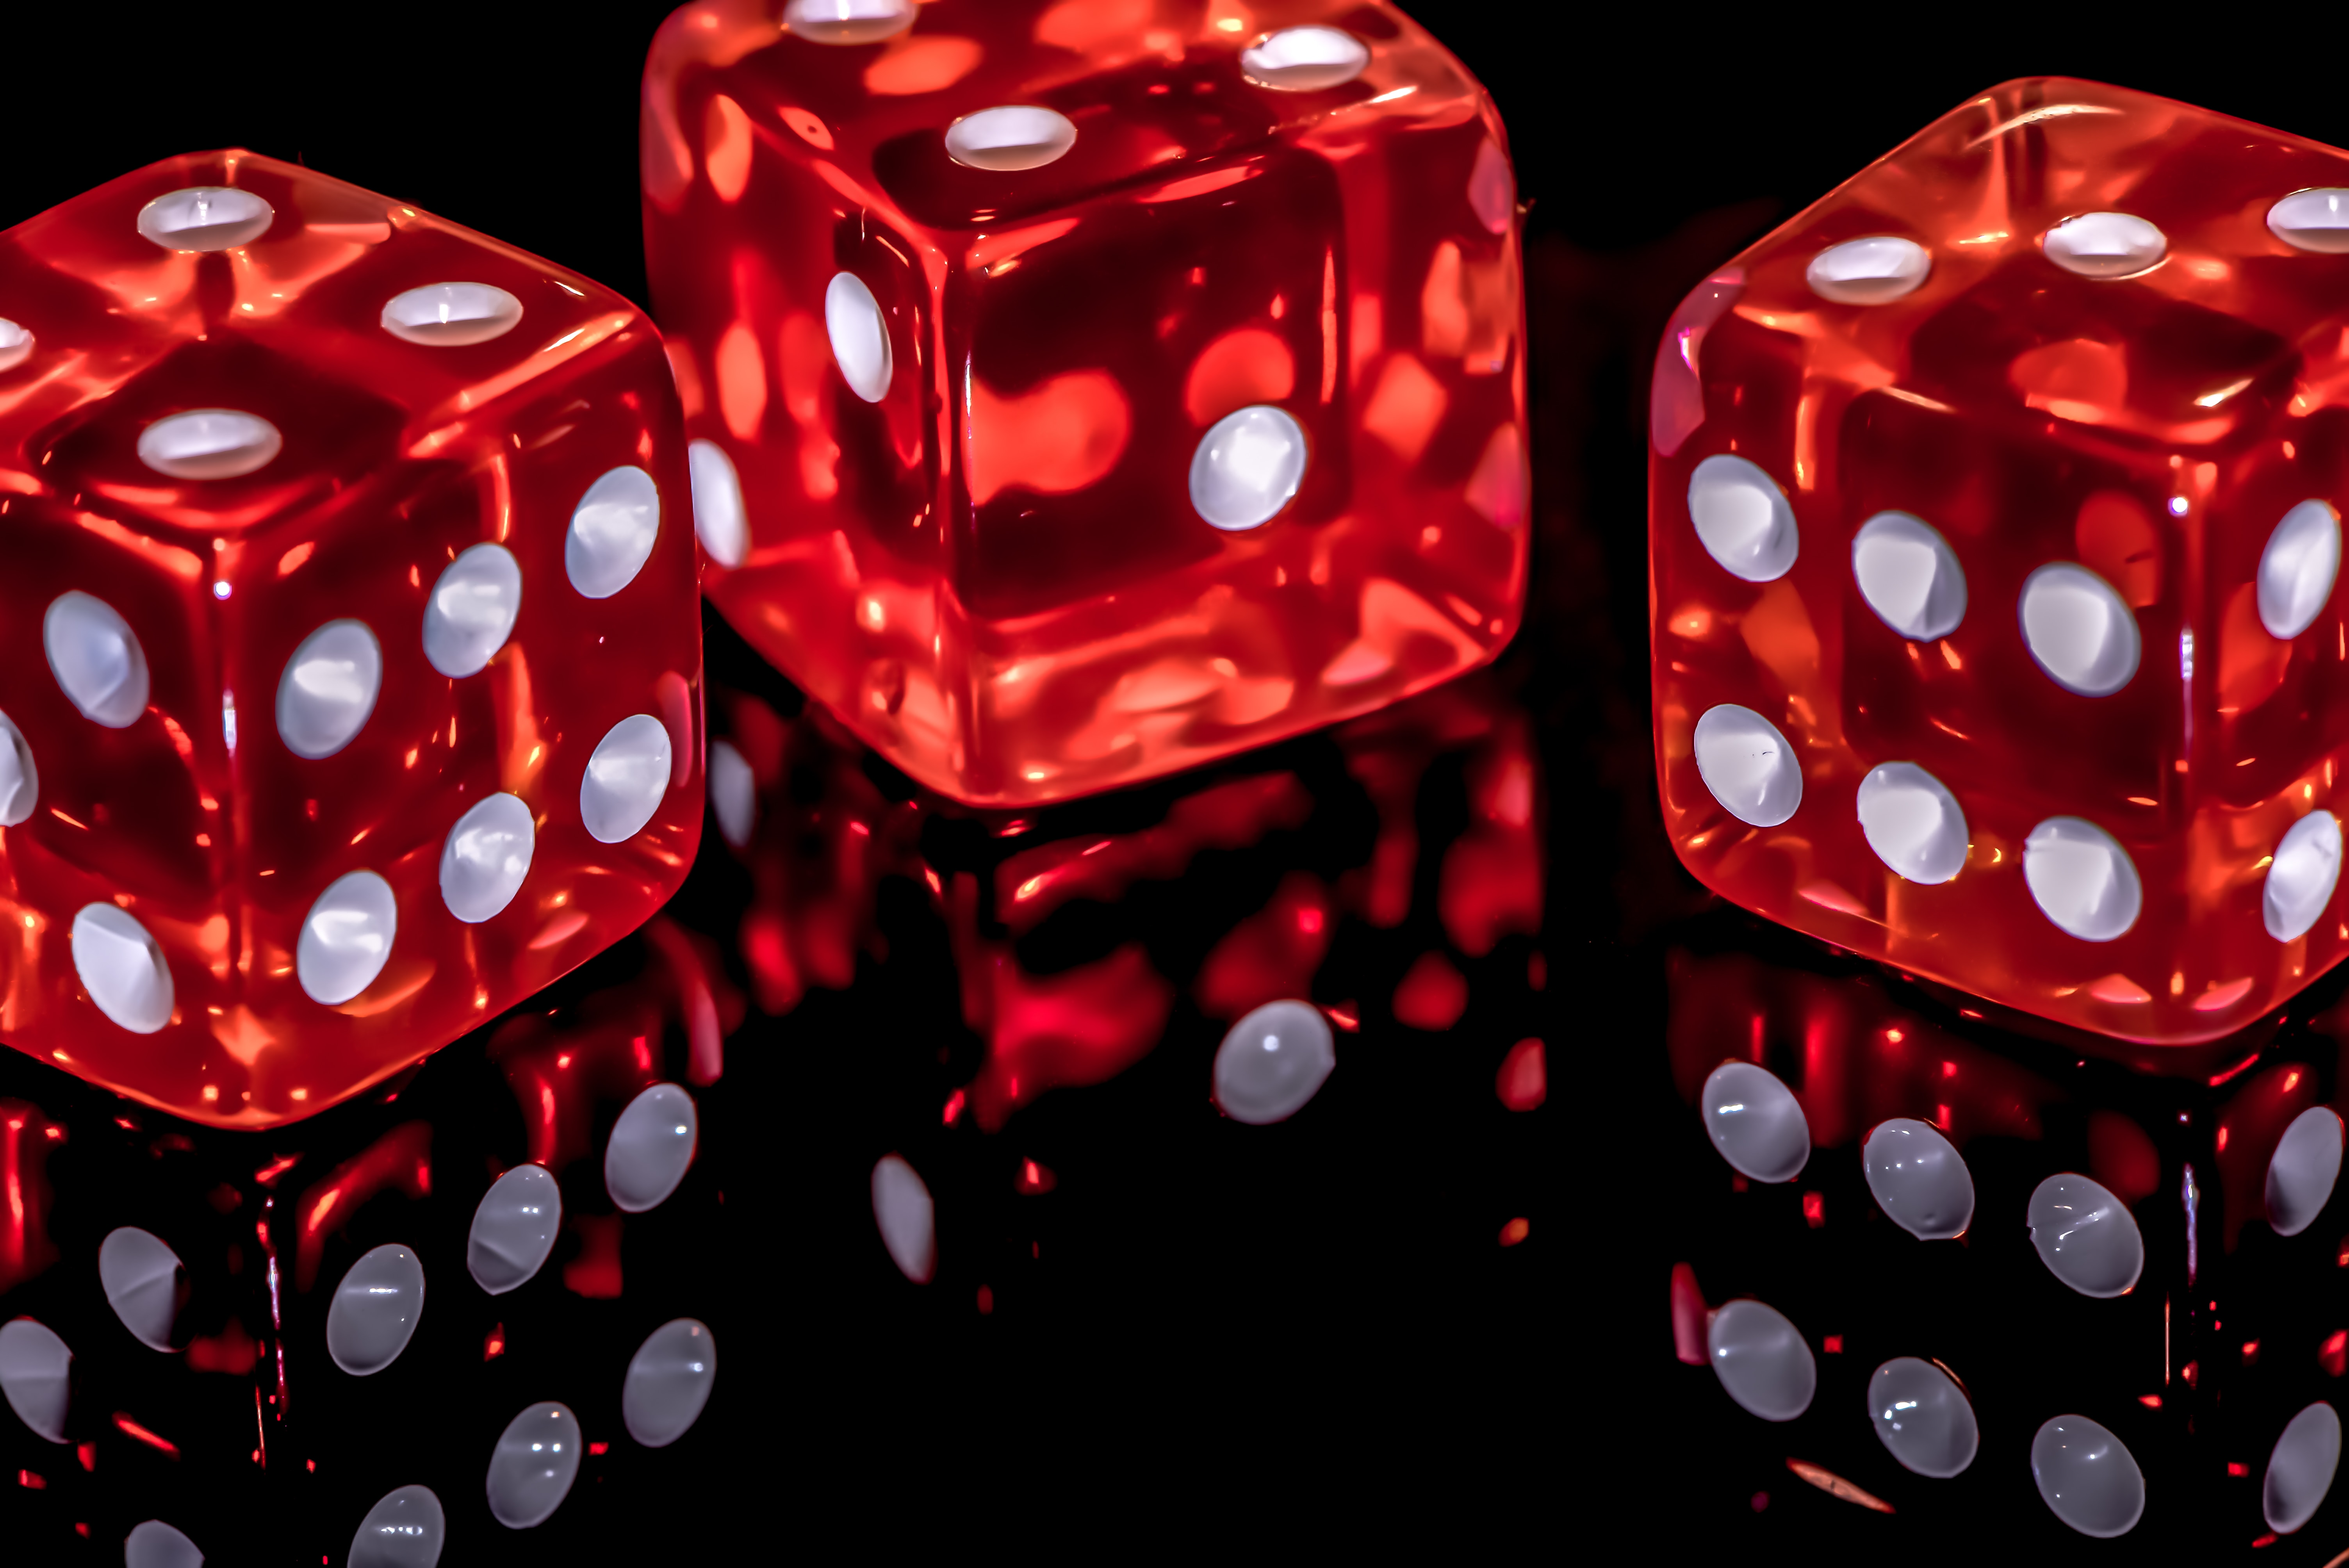
\includegraphics[height=\paperheight]{title.jpg}}

\def\subsectionname{}

% enumerate global settings
\setlist[enumerate,1]{label=\arabic*.}
\setlist[enumerate,2]{label=\alph*)}

% custom colors %
\definecolor{DarkRed}{HTML}{260104}
\definecolor{LightRed}{HTML}{8C031C}
\definecolor{Red}{HTML}{590212}
\definecolor{Gray}{HTML}{4D4A59}
\definecolor{DarkBrown}{HTML}{0D0000}
\colorlet{tPrim}{DarkRed}
\colorlet{tTheme}{LightRed}
\colorlet{tSec}{LightRed}
\colorlet{tAccent}{Gray}
\colorlet{tText}{DarkBrown}

\newcommand{\clr}{\textcolor{BrickRed}}
\newcommand{\clb}{\textcolor{RoyalBlue}}
\newcommand{\clg}{\textcolor{ForestGreen}}
\newcommand{\clm}{\textcolor{Magenta}}

\DeclareMathOperator{\var}{Var}

\tcbset{
 boxsep=7pt,
 fonttitle=\sc,
 colframe=tGreyBg,
 colframe=tTheme,
 boxrule=1pt
}

\begin{document}
\titleframe

% \section{Probabilistic Intuition}
% \label{sec:probabilistic-intuition}
%
% \begin{frame}
%  \frametitle{What Is Chance?}
%  Imagine you have 9 balls of different colours.\pause
%  \begin{center}
%   \begin{tikzpicture}
%    \foreach \x in {0,1,2} {
%     \foreach \y in {0,1,2} {
%      \tkzDefPoint(\x,\y){\x\y}
%     }
%    }
%    \tkzDrawPoints[color=BrickRed](00,12,20,21)
%    \tkzDrawPoints[color=RoyalBlue](01,11,22)
%    \tkzDrawPoints[color=ForestGreen](02,10)
%   \end{tikzpicture}
%  \end{center}
%  \pause
%  \begin{itemize}
%   \item If you pick a ball \alert{at random}, what colour is it most likely to
%    be?\pause
%   \item How many times more likely is picking a \clr{red} ball than picking a
%    \clg{green} ball?\pause
%  \end{itemize}
% \end{frame}
%
% \begin{frame}
%  \frametitle{Quantifying Probability}
%  \begin{tcolorbox}[title=Probability]
%   A \alert{probability} is a number between $0$ and $1$ measuring how
%   \alert{likely} is something to happen.
%  \end{tcolorbox}
% \end{frame}
%
% \begin{frame}
%  \frametitle{Quantifying Probability -- Example}
%  In our example of 9 balls
%  \begin{center}
%   \vspace*{-2em}
%   \begin{tikzpicture}
%    \foreach \x in {0,1,2} {
%     \foreach \y in {0,1,2} {
%      \tkzDefPoint(\x,\y){\x\y}
%     }
%    }
%    \tkzDrawPoints[color=BrickRed](00,12,20,21)
%    \tkzDrawPoints[color=RoyalBlue](01,11,22)
%    \tkzDrawPoints[color=ForestGreen](02,10)
%   \end{tikzpicture}
%  \end{center}
%  what is the probability of picking a ball of a specific colour?\pause
%  \begin{itemize}
%   \item For \clr{red}, it's $4 / 9$.
%   \item For \clb{blue}, it's $3 / 9$.
%   \item For \clg{green}, it's $2 / 9$.
%  \end{itemize}\pause
%  The probabilities above \alert{sum up to $1$} because I am certain to pick
%  \emph{some} ball.
% \end{frame}
%
% \begin{frame}
%  \frametitle{Quantifying Probability -- Example}
%  We'll all the outcome of a random choice, a \alert{random variable} and
%  typically write it as $X$.\pause\\
%  A random variable always lies in the set of all possible outcomes.\pause\\
%  In this case, the variable $X$ must lie in the set of possible colours,
%  $\{\clr{\text{red}},\clb{\text{blue}},\clg{\text{green}}\}$.\pause\\
%  We'll write the probability that $X$ is equal to one of the elements in the set
%  as $P(X=\text{colour})$.\pause\\
%  So, for the 9-ball example from before, we would have
%  \[
%   P(X=\text{\clr{red}}) = \frac{4}{9}, \quad P(X=\text{\clb{blue}}) =
%   \frac{3}{9}, \quad P(X=\text{\clg{green}}) = \frac{2}{9}.
%  \]
% \end{frame}
%
% \begin{frame}
%  \frametitle{Calculating Probability}
%  In the case the set of outcomes is \alert{finite}, the probability of $X$ being
%  one of the possible outcomes is always\pause
%  \begin{tcolorbox}
%   \[
%    P(X \in S) = \frac{|S|}{|O|},
%   \]
%  \end{tcolorbox}
%   where $S$ is a certain subset of $O$ -- all the possible outcomes.
% \end{frame}
%
% \begin{frame}
%  \frametitle{Calculating Probability -- Example}
%  We'll describe our 9-ball example more formally.\pause\\
%  We'll assign the balls number from $1$ to $9$. The set of all possible outcomes
%  of picking a random ball is then
%  \[
%   O = \{1,2,3,4,5,6,7,8,9\}.
%  \]
%  \begin{center}
%   \begin{tikzpicture}
%    \foreach \x in {0,1,2} {
%     \foreach \y in {0,1,2} {
%      \tkzDefPoint(\x,\y){\x\y}
%     }
%    }
%    \tkzDrawPoints[color=BrickRed](00,12,20,21)
%    \tkzDrawPoints[color=RoyalBlue](01,11,22)
%    \tkzDrawPoints[color=ForestGreen](02,10)
%
%    \tkzLabelPoint[above,color=BrickRed](00){$7$}
%    \tkzLabelPoint[above,color=BrickRed](12){$2$}
%    \tkzLabelPoint[above,color=BrickRed](20){$9$}
%    \tkzLabelPoint[above,color=BrickRed](21){$6$}
%
%    \tkzLabelPoint[above,color=RoyalBlue](01){$4$}
%    \tkzLabelPoint[above,color=RoyalBlue](11){$5$}
%    \tkzLabelPoint[above,color=RoyalBlue](22){$3$}
%
%    \tkzLabelPoint[above,color=ForestGreen](02){$1$}
%    \tkzLabelPoint[above,color=ForestGreen](10){$8$}
%   \end{tikzpicture}
%  \end{center}
% \end{frame}
%
% \begin{frame}
%  \frametitle{Calculating Probability -- Example}
%  \begin{center}
%   \vspace*{-1em}
%   \begin{tikzpicture}
%    \foreach \x in {0,1,2} {
%     \foreach \y in {0,1,2} {
%      \tkzDefPoint(\x,\y){\x\y}
%     }
%    }
%    \tkzDrawPoints[color=BrickRed](00,12,20,21)
%    \tkzDrawPoints[color=RoyalBlue](01,11,22)
%    \tkzDrawPoints[color=ForestGreen](02,10)
%
%    \tkzLabelPoint[above,color=BrickRed](00){$7$}
%    \tkzLabelPoint[above,color=BrickRed](12){$2$}
%    \tkzLabelPoint[above,color=BrickRed](20){$9$}
%    \tkzLabelPoint[above,color=BrickRed](21){$6$}
%
%    \tkzLabelPoint[above,color=RoyalBlue](01){$4$}
%    \tkzLabelPoint[above,color=RoyalBlue](11){$5$}
%    \tkzLabelPoint[above,color=RoyalBlue](22){$3$}
%
%    \tkzLabelPoint[above,color=ForestGreen](02){$1$}
%    \tkzLabelPoint[above,color=ForestGreen](10){$8$}
%   \end{tikzpicture}
%   \vspace*{-1em}
%  \end{center}
%  We'll form three subsets of $O$:
%  \begin{align*}
%   \clr{R} &= \{\clr{2},\clr{6},\clr{7},\clr{9}\},\\
%   \clb{B} &= \{\clb{3},\clb{4},\clb{5}\},\\
%   \clg{G} &= \{\clg{1},\clg{8}\}.
%  \end{align*}\pause
%  We can use the formula from before to calculate the probability that $X$ will
%  be a \clg{green} ball:
%  \[
%   P(X \in \clg{G}) = \frac{|\clg{G}|}{|O|} = \frac{2}{9}.
%  \]
% \end{frame}
%
% \section{Probability Equations}
% \label{sec:probability-equations}
%
% \begin{frame}
%  \frametitle{Sums of Probabilities}
%  What if I asked about the probability that the ball I pick is \clr{red} or
%  \clb{blue}?\pause\\
%  We can literally use the same formula as before. Now, the set of outcomes we're
%  interested in is $\clr{R} \cup \clb{B}$ and so\pause
%  \[
%   P(X \in \clr{R} \cup \clb{B}) = \frac{|\clr{R} \cup \clb{B}|}{|O|} =
%   \frac{|\clr{R}| + |\clb{B}|}{|O|} = \frac{4+3}{9} = \frac{7}{9}.
%  \]
%  \pause
%  However, this example cannot be easily generalized. We'll see why.
% \end{frame}
%
% \begin{frame}
%  \frametitle{Sums of Probabilities -- Counterexample}
%  Suppose we're instead choosing from a set of numbers between $1$ and
%  $20$.\pause\\
%  We want to calculate the probability that a randomly picked number is
%  \alert{even or divisible by $5$}.\pause\\
%  So, we have
%  \begin{align*}
%   O &= \{1,2,\ldots,20\},\\
%   E &= \{2,4,6,\ldots,20\},\\
%   F &= \{5,10,15,20\}.
%  \end{align*}\pause
%  and we want to figure out the probability $P(X \in E \cup F)$.
% \end{frame}
%
% \begin{frame}
%  \frametitle{Sums of Probabilities -- Counterexample}
%  Let's try to use the same formula as before:
%  \[
%   P(X \in E \cup F) = \frac{|E \cup F|}{|O|} \overset{??}{=} \frac{|E| +
%   |F|}{|O|} = \frac{10 + 4}{20} = \frac{14}{20}.
%  \]\pause
%  This doesn't quite add up.\pause\\
%  If we count such numbers by hand, we get the set
%  \[
%   \{2,4,5,6,8,10,12,14,15,16,18,20\}.
%  \]
%  \pause
%  There's \alert{only 12 of them}.\pause\\
%  The problem is that \alert{we counted the numbers 10 and 20 twice}!\pause\\
%  So, to get the size of $E \cup F$, we cannot just add the size of $E$ to the
%  size of $F$ but we also have to subtract the elements that appear twice -- the
%  size of $E \cap F$.
% \end{frame}
%
% \begin{frame}
%  \frametitle{Sums of Probabilities -- Formula}
%  The previous example applies in general. If $A,B$ are two subsets of the set of
%  outcomes, $O$, then\pause
%  \begin{tcolorbox}
%   \[
%    P(X \in A \cup B) = \frac{|A \cup B|}{|O|} = \frac{|A| + |B| - |A \cap
%    B|}{|O|}.
%   \]
%  \end{tcolorbox}
% \end{frame}
%
% \begin{frame}
%  \frametitle{Sums of Probabilities -- Formula}
%  We have a formula for two sets but how about three sets? Four sets? Million
%  sets?\pause\\
%  We need a \alert{general formula} to calculate the size
%  \[
%   |A_1 \cup A_2 \cup \ldots \cup A_n|
%  \]
%  where $A_1,A_2,\ldots,A_n$ are any sets.\pause\\
%  Such a formula is widely known as the \alert{principle of inclusion and
%  exclusion}.
% \end{frame}
%
% \begin{frame}
%  \frametitle{Principle of Inclusion and Exclusion -- Example}
%  Let's consider the following setup: There are three language groups -- English,
%  French and German.\pause
%  \begin{itemize}
%   \item 40 people speak English, 23 speak German and 11 speak French.\pause
%   \item 10 people speak both English and German, 5 speak both English and French
%    and only 3 speak both German and French.\pause
%   \item Finally, just one person speaks all three languages.
%  \end{itemize}
%  \pause
%  How many people speak at least one language?
% \end{frame}
%
% \begin{frame}
%  \frametitle{Principle of Inclusion and Exclusion -- Example}
%  Let's tackle this formally.\pause\\
%  Label the three language groups $E$, $F$ and $G$. The setup from the previous
%  slide can be summarized as
%  \begin{center}
%   \begin{tabular}{ccccccc}
%    $|E|$ & $|F|$ & $|G|$ & $|E \cap F|$ & $|E \cap G|$ & $|F \cap G|$ & $|E \cap
%    F \cap G|$\\
%    \midrule
%    40 & 11 & 23 & 5 & 10 & 3 & 1
%   \end{tabular}
%  \end{center}
%  \pause
%  We're trying to calculate $|E \cup F \cup G|$.
% \end{frame}
%
% \begin{frame}
%  \frametitle{Principle of Inclusion and Exclusion -- Example}
%  Let's picture the problem first.\pause\\
%  When working with sets, Venn diagrams are often a great choice.
%  \begin{center}
%   \begin{tikzpicture}
%    \begin{scope}[transparency group]
%     \begin{scope}[blend mode=screen]
%      \filldraw[fill=BrickRed,draw=Black] (90:0.6) circle[radius=1];
%      \filldraw[fill=RoyalBlue,draw=Black] (210:0.6) circle[radius=1];
%      \filldraw[fill=ForestGreen,draw=Black] (330:0.6) circle[radius=1];
%
%      \node[BrickRed] at (90:2) {\Large $E$};
%      \node[RoyalBlue] at (210:2) {\Large $F$};
%      \node[ForestGreen] at (330:2) {\Large $G$};
%     \end{scope}
%    \end{scope}
%   \end{tikzpicture}
%  \end{center}
%  \pause
%  There are 7 regions in total (differentiated by colour) in this picture,
%  corresponding to the 7 sets in the previous slide.
% \end{frame}
%
% \begin{frame}
%  \frametitle{Principle of Inclusion and Exclusion -- Example}
%  \begin{center}
%   \begin{tikzpicture}
%    \begin{scope}[transparency group]
%     \begin{scope}[blend mode=screen]
%      \filldraw[fill=BrickRed,draw=Black] (90:0.6) circle[radius=1];
%      \filldraw[fill=RoyalBlue,draw=Black] (210:0.6) circle[radius=1];
%      \filldraw[fill=ForestGreen,draw=Black] (330:0.6) circle[radius=1];
%
%      \node[BrickRed] at (90:2) {\Large $E$};
%      \node[RoyalBlue] at (210:2) {\Large $F$};
%      \node[ForestGreen] at (330:2) {\Large $G$};
%     \end{scope}
%    \end{scope}
%   \end{tikzpicture}
%  \end{center}
%  What we need to count is the total number of elements inside this entire
%  shape.\pause\\
%  Let's start by counting the number of elements in each of the regions
%  separately and assign numbers to regions corresponding to \alert{how many times
%  we've counted all the elements in that region}.
% \end{frame}
%
% \begin{frame}
%  \frametitle{Principle of Inclusion and Exclusion -- Example}
%  \begin{center}
%   \begin{tikzpicture}
%    \begin{scope}[transparency group]
%     \begin{scope}[blend mode=screen]
%      \filldraw[fill=BrickRed,draw=Black] (90:0.6) circle[radius=1];
%      \filldraw[fill=RoyalBlue,draw=Black] (210:0.6) circle[radius=1];
%      \filldraw[fill=ForestGreen,draw=Black] (330:0.6) circle[radius=1];
%
%      \node[BrickRed] at (90:2) {\Large $E$};
%      \node[RoyalBlue] at (210:2) {\Large $F$};
%      \node[ForestGreen] at (330:2) {\Large $G$};
%
%      \node[White] at (90:1) {\Large $\mathbf{1}$};
%      \node[White] at (210:1) {\Large $\mathbf{1}$};
%      \node[White] at (330:1) {\Large $\mathbf{1}$};
%      \node[White] at (150:0.7) {\Large $\mathbf{2}$};
%      \node[White] at (270:0.7) {\Large $\mathbf{2}$};
%      \node[White] at (30:0.7) {\Large $\mathbf{2}$};
%      \node[White] at (0,0) {\Large $\mathbf{3}$};
%     \end{scope}
%    \end{scope}
%   \end{tikzpicture}
%  \end{center}
%  \[
%   |E \cup F \cup G| = |E| + |F| + |G| \ldots
%  \]
% \end{frame}
%
% \begin{frame}
%  \frametitle{Principle of Inclusion and Exclusion -- Example}
%  \begin{center}
%   \begin{tikzpicture}
%    \begin{scope}[transparency group]
%     \begin{scope}[blend mode=screen]
%      \filldraw[fill=BrickRed,draw=Black] (90:0.6) circle[radius=1];
%      \filldraw[fill=RoyalBlue,draw=Black] (210:0.6) circle[radius=1];
%      \filldraw[fill=ForestGreen,draw=Black] (330:0.6) circle[radius=1];
%
%      \node[BrickRed] at (90:2) {\Large $E$};
%      \node[RoyalBlue] at (210:2) {\Large $F$};
%      \node[ForestGreen] at (330:2) {\Large $G$};
%
%      \node[White] at (90:1) {\Large $\mathbf{1}$};
%      \node[White] at (210:1) {\Large $\mathbf{1}$};
%      \node[White] at (330:1) {\Large $\mathbf{1}$};
%      \node[White] at (150:0.7) {\Large $\mathbf{1}$};
%      \node[White] at (270:0.7) {\Large $\mathbf{1}$};
%      \node[White] at (30:0.7) {\Large $\mathbf{1}$};
%      \node[White] at (0,0) {\Large $\mathbf{0}$};
%     \end{scope}
%    \end{scope}
%   \end{tikzpicture}
%  \end{center}
%  \[
%   |E \cup F \cup G| = |E| + |F| + |G| - |E \cap F| - |E \cap G| - |F \cap G|
%  \]
% \end{frame}
%
% \begin{frame}
%  \frametitle{Principle of Inclusion and Exclusion -- Example}
%  \begin{center}
%   \begin{tikzpicture}
%    \begin{scope}[transparency group]
%     \begin{scope}[blend mode=screen]
%      \filldraw[fill=BrickRed,draw=Black] (90:0.6) circle[radius=1];
%      \filldraw[fill=RoyalBlue,draw=Black] (210:0.6) circle[radius=1];
%      \filldraw[fill=ForestGreen,draw=Black] (330:0.6) circle[radius=1];
%
%      \node[BrickRed] at (90:2) {\Large $E$};
%      \node[RoyalBlue] at (210:2) {\Large $F$};
%      \node[ForestGreen] at (330:2) {\Large $G$};
%
%      \node[White] at (90:1) {\Large $\mathbf{1}$};
%      \node[White] at (210:1) {\Large $\mathbf{1}$};
%      \node[White] at (330:1) {\Large $\mathbf{1}$};
%      \node[White] at (150:0.7) {\Large $\mathbf{1}$};
%      \node[White] at (270:0.7) {\Large $\mathbf{1}$};
%      \node[White] at (30:0.7) {\Large $\mathbf{1}$};
%      \node[White] at (0,0) {\Large $\mathbf{1}$};
%     \end{scope}
%    \end{scope}
%   \end{tikzpicture}
%  \end{center}
%  \[
%   |E \cup F \cup G| = |E| + |F| + |G| - |E \cap F| - |E \cap G| - |F \cap G| +
%   |E \cap F \cap G|.
%  \]
% \end{frame}
%
% \begin{frame}
%  \frametitle{Principle of Inclusion and Exclusion -- Example}
%  \[
%   |E \cup F \cup G| = |E| + |F| + |G| - |E \cap F| - |E \cap G| - |F \cap G| +
%   |E \cap F \cap G|.
%  \]
%  Apply this formula to our example with language groups gives
%  \[
%   |E \cup F \cup G| = 40 + 11 + 23 - 5 - 10 - 3 + 1 = 57.
%  \]
%  \pause
%  So, 57 people speak at least one language.
% \end{frame}
%
% \begin{frame}
%  \frametitle{Principle of Inclusion and Exclusion -- Formula}
%  The previous example can be generalized to any number of sets.\pause\\
%  The basic idea is
%  \begin{enumerate}
%   \item Add the sizes of all the sets.\pause
%   \item Subtract the size of all two-set intersections.\pause
%   \item Add the sizes of all three-set intersections.\pause
%   \item Subtract the sizes of all four-set intersections.\pause
%   \item ...
%  \end{enumerate}
% \end{frame}
%
% \begin{frame}
%  \frametitle{Principle of Inclusion and Exclusion -- Formula}
%  If $A_1,A_2,\ldots,A_n$ are sets with $n \in \mathbb{N}$, then
%  \begin{tcolorbox}[top=-\parskip,title=Principle of Inclusion and Exclusion]
%   \begin{align*}
%    |A_1 \cup A_2 \cup \ldots A_n| &= |A_1| + |A_2| + |A_3| + \ldots + |A_n|\\
%                                   &- |A_1 \cap A_2| - \ldots - |A_1 \cap A_n| -
%                                   |A_2 \cap A_3| - \ldots - |A_{n-1} \cap A_n|\\
%                                   &+ |A_1 \cap A_2 \cap A_3| + \ldots + |A_1
%                                   \cap A_2 \cap A_n| + \ldots |A_{n-2} \cap
%                                   A_{n-1} \cap A_n|\\
%                                   & \hspace*{3em} \vdots \\
%                                   & + (-1)^{n} |A_1 \cap A_2 \cap \ldots \cap
%                                   A_n|.
%   \end{align*}
%  \end{tcolorbox}
%  \pause
%  The $(-1)^{n}$ only means that if $n$ is odd, then I subtract the last term,
%  and I add it if $n$ is even.
% \end{frame}
%
% \begin{frame}
%  \frametitle{Principle of Inclusion and Exclusion -- Problems}
%  Probabilistic problems requiring the \alert{principle of exclusion and
%  inclusion} are those with multiple desirable outcomes.\pause\\
%  Let's start with something familiar:
%  \begin{center}
%   \emph{Out of the numbers 1 to 100, what is the probability that a randomly
%   picked number is a multiple of 2, 3 or 7?}
%  \end{center}
%  \pause
%  Let's define the sets
%  \[
%   E = \{\text{multiples of 2}\}, \quad T = \{\text{multiples of 3}\}, \quad S =
%   \{\text{multiples of 7}\}
%  \]
%  \pause
%  and
%  \[
%   O = \{1,2,\ldots,100\}.
%  \]
% \end{frame}
%
% \begin{frame}
%  \frametitle{Principle of Inclusion and Exclusion -- Problems}
%  We're figuring out the probability
%  \[
%   P(X \in E \cup T \cup S) = \frac{|E \cup T \cup S|}{|O|}.
%  \]
%  \pause
%  Using the \alert{inclusion-exclusion principle}, we count
%  \begin{align*}
%   |E \cup T \cup S| &= |E| + |T| + |S| - \underbrace{|E \cap
%   T|}_{\text{multiples of $6$}} - \underbrace{|E \cap S|}_{\text{multiples of
%   $14$}} - \underbrace{|T \cap S|}_{\text{multiples of $21$}} + \underbrace{|E \cap T \cap
%   S|}_{\text{multiples of $42$}} \\
%                     &= 50 + 33 + 14 - 16 - 7 - 4 + 2 = 72.
%  \end{align*}
%  \pause
%  So,
%  \[
%   P(X \in E \cup T \cup S) = \frac{72}{100}.
%  \]
% \end{frame}
%
% \begin{frame}
%  \frametitle{Principle of Inclusion and Exclusion -- Problems}
%  Given two circles and a triangle in the plane, what's the maximum number of
%  points that can belong to at least two of these shapes?\pause\\
%  Let's label the circles $C_1,C_2$ and the triangle $T$. \pause
%  We're interested in points that lie in \alert{at least one} of the sets $C_1
%  \cap C_2, C_1 \cap T$ and $C_2 \cap T$.\pause\\
%  In other words, we want to determine the maximum size of
%  \[
%   |(C_1 \cap C_2) \cup (C_1 \cap T) \cup (C_2 \cap T)|.
%  \]
%  \pause
%  The maximum number of points
%  \begin{itemize}
%   \item two circles can share is $2$. So, let's set $|C_1 \cap C_2| = 2$.
%   \pause
%   \item circle and a triangle can share is $6$. So $|C_1 \cap T| = |C_2 \cap T|
%    = 6$.
%   \pause
%   \item all three objects share is zero if the number of intersections is
%    maximized. So $|C_1 \cap C_2 \cap T| = 0$.
%  \end{itemize}
% \end{frame}
%
% \begin{frame}
%  \frametitle{Principle of Inclusion and Exclusion -- Problems}
%  Let's apply the inclusion-exclusion principle. We get
%  \begin{align*}
%   &|(C_1 \cap C_2) \cup (C_1 \cap T) \cup (C_2 \cup T)| \\
%   &= |C_1 \cap C_2| + |C_1 \cap T| + |C_2 \cap T| \\
%                                                        &- |(C_1 \cap C_2) \cap
%                                                        (C_1 \cap T)| - |(C_1
%                                                        \cap C_2) \cap (C_2 \cap
%                                                        T)| 
%                                                        - |(C_1 \cap T) \cap
%                                                        (C_2 \cap T)| \\
%                                                        &+ |(C_1 \cap C_2) \cap
%                                                        (C_1 \cap T) \cap (C_2
%                                                        \cap T)|.
%  \end{align*}
% \end{frame}
%
% \begin{frame}
%  \frametitle{Principle of Inclusion and Exclusion -- Problems}
%  This is less scary than it looks. Actually, most of the intersections there are
%  one and the same. Really,
%  \begin{align*}
%   (C_1 \cap C_2) \cap (C_1 \cap T) &= C_1 \cap C_2 \cap T \\
%   (C_1 \cap C_2) \cap (C_2 \cap T) &= C_1 \cap C_2 \cap T \\
%   (C_1 \cap T) \cap (C_2 \cap T) &= C_1 \cap C_2 \cap T \\
%   (C_1 \cap C_2) \cap (C_1 \cap T) \cap (C_2 \cap T) &= C_1 \cap C_2 \cap T.
%  \end{align*}
%  \pause
%  So, the previous expression just ends up being
%  \[
%   |C_1 \cap C_2| + |C_1 \cap T| + |C_2 \cap T| - 2 \cdot |C_1 \cap C \cap T| = 2
%   + 6 + 6 - 2 \cdot 0 = 14.
%  \]
%  
% \end{frame}
%
% \section{Events}
% \label{sec:events}
%
% \begin{frame}
%  \frametitle{What Is An Event?}
%  Formally, an \alert{event} is just an element which \alert{has some
%  probability}.\\
%  However, we typically think of events as \alert{things that have some chance of
%  happening}.\\
%  For example
%  \begin{itemize}
%   \item the fact that a random variable $X$ lies in some set is an event.
%   \pause
%   \item the fact that a randomly chosen ball has a specific colour is an event.
%   \pause
%   \item the fact that the universe ends today at midnight is an event.
%  \end{itemize}
% \end{frame}
%
% \begin{frame}
%  \frametitle{Operations On Events}
%  Ultimately, an event is \alert{logical sentence}, meaning it's a sentence which
%  is either \alert{true} or \alert{false}.\pause\\
%  Logical sentences can be negated (written as $\neg $) and joined together using
%  logical conjunctions\pause\\
%  \begin{itemize}
%   \item \alert{and} (written as $ \wedge $),
%   \pause
%   \item \alert{or} (written as $ \vee $).
%  \end{itemize}
%  \pause
%  We want to understand how to calculate $P(\neg A),P(A \wedge B),P(A \vee B)$
%  for two events $A,B$ whose probabilities we know.
% \end{frame}
%
% \begin{frame}
%  \frametitle{Negating Events}
%  Suppose we have an event $A = \text{`It's going to rain in 5 minutes.'}$ with
%  probability 0.2.\pause\\
%  What's the probability of $\neg A$?\pause\\
%  Quite naturally, it's 0.8 because it either is going to rain or it's not. The
%  total of the probabilities of those two events has to be 1.\pause
%  \begin{tcolorbox}[title=Negation Formula]
%   If $A$ is an event with probability $P(A) = p$, then
%   \[
%    P(\neg A) = 1 - p.
%   \]
%  \end{tcolorbox}
% \end{frame}
%
% \begin{frame}
%  \frametitle{Independent and Incompatible Events}
%  Two events are called \alert{independent} if the result of one event doesn't at
%  all influence the result of the other.\pause\\
%  For example, two tosses of a coin are independent.\pause\\
%  \vspace{2\parskip}
%  \hrule
%  Two events are called \alert{incompatible} if they cannot \emph{both}
%  happen.\pause\\
%  For example, the events `I'm going to spend vacation in Florida.' and `I'm
%  going to spend vacation in Spain.' are incompatible.\pause\\
%  An event is always incompatible with its own negation.
% \end{frame}
%
% \begin{frame}
%  \frametitle{Conjunction of Events}
%  \begin{tcolorbox}[title=Conjunction Formula]
%   If $A,B$ are two \alert{independent} events, then
%   \[
%    P(A \wedge B) = P(A) \cdot P(B).
%   \]
%  \end{tcolorbox}
%  \pause
%  If the two events are \alert{dependent}, then calculating the probability of
%  their conjunction is much more difficult. We'll need \emph{conditional
%  probability} for that.
% \end{frame}
%
% \begin{frame}
%  \frametitle{Disjunction of Events}
%  The disjunction formula for events is really just the inclusion-exclusion
%  principle.\pause\\
%  \begin{tcolorbox}[title=Disjunction Formula]
%   If $A,B$ are any events, then
%   \[
%    P(A \vee B) = P(A) + P(B) - P(A \wedge B).
%   \]
%  \end{tcolorbox}
%  \pause
%  If $A,B$ are \alert{incompatible}, then $P(A \wedge B) = 0$ and the formula
%  above becomes $P(A \vee B) = P(A) + P(B)$.
% \end{frame}
%
% \begin{frame}
%  \frametitle{Conditional Probability}
%  Conditional is the probability of an event happening \alert{given another event
%  has already happened}.
%  \pause
%  \begin{tcolorbox}[title=Conditional Probability]
%   If $A,B$ are events, then
%   \[
%    P(A \mid B)
%   \]
%   is the probability that $A$ happens supposing $B$ has already happened.
%  \end{tcolorbox}
% \end{frame}
%
% \begin{frame}
%  \frametitle{Conditional Probability -- Example}
%  \begin{center}
%   \begin{tikzpicture}
%    \foreach \x in {0,1,2} {
%     \foreach \y in {0,1,2} {
%      \tkzDefPoint(\x,\y){\x\y}
%     }
%    }
%    \tkzDrawPoints[color=BrickRed](00,12,20,21)
%    \tkzDrawPoints[color=RoyalBlue](01,11,22)
%    \tkzDrawPoints[color=ForestGreen](02,10)
%   \end{tikzpicture}
%  \end{center}
%  In our balls example, suppose
%  \begin{itemize}
%   \item $A$ is the event that the \alert{second} randomly chosen ball is red.
%   \item $B$ is the event that the \alert{first} randomly chosen ball is red.
%  \end{itemize}
%  \pause
%  What is the probability $P(A \mid B)$?
% \end{frame}
%
% \begin{frame}
%  \frametitle{Conditional Probability -- Example}
%  \begin{center}
%   \begin{tikzpicture}
%    \foreach \x in {0,1,2} {
%     \foreach \y in {0,1,2} {
%      \tkzDefPoint(\x,\y){\x\y}
%     }
%    }
%    \tkzDrawPoints[color=BrickRed](00,12,20,21)
%    \tkzDrawPoints[color=RoyalBlue](01,11,22)
%    \tkzDrawPoints[color=ForestGreen](02,10)
%    \tkzDrawPoint[color=Black,shape=cross out,size=10,thick](21)
%   \end{tikzpicture}
%  \end{center}
%  If $B$ has happened, then there are only 3 red balls left in the set of 8
%  balls.\pause\\
%  Therefore $P(A \mid B) = 3 / 8$.
% \end{frame}
%
% \begin{frame}
%  \frametitle{Conditional Probability \& Conjunction}
%  We can use conditional probability to compute $P(A \wedge B)$ for \alert{any}
%  events $A$ and $B$, not necessarily independent.\pause\\
%  If, for example, $A$ is dependent on $B$, then $A$ can \alert{only happen if
%  $B$ happened as well}. \pause
%  In other words, the probability that $A \wedge B$ happens is the probability
%  that $B$ happens times the probability that $A$ happens \alert{supposing $B$
%  happened}.
%  \pause
%  \begin{tcolorbox}[title=Event Conjunction Formula]
%   If $A,B$ are \alert{any} events, then
%   \[
%    P(A \wedge B) = P(B) \cdot P(A \mid B) = P(A) \cdot P(B \mid A).
%   \]
%  \end{tcolorbox}
% \end{frame}
%
% \begin{frame}
%  \frametitle{Conditional Probability \& Conjunction}
%  \begin{center}
%   \begin{tikzpicture}
%    \foreach \x in {0,1,2} {
%     \foreach \y in {0,1,2} {
%      \tkzDefPoint(\x,\y){\x\y}
%     }
%    }
%    \tkzDrawPoints[color=BrickRed](00,12,20,21)
%    \tkzDrawPoints[color=RoyalBlue](01,11,22)
%    \tkzDrawPoints[color=ForestGreen](02,10)
%   \end{tikzpicture}
%  \end{center}
%  The event $A \wedge B$ in the ball example means that the first two randomly
%  chosen balls are red.\pause\\
%  We know that $P(B) = 4 / 9$ and $P(A \mid B) = 3 / 8$. Therefore,
%  \[
%   P(A \wedge B) = P(B) \cdot P(A \mid B) = \frac{4}{9} \cdot \frac{3}{8} =
%   \frac{1}{6}.
%  \]
% \end{frame}
% \begin{frame}
%  \frametitle{Conditional Probability -- Examples}
%  Suppose the probability that a woman will live to at least 70 years is $0.7$
%  and that she will live to at least 80 years is $0.55$. What is the probability
%  that she will live to 80 supposing she has already turned 70?\pause\\
%  \vspace*{1em}
%  \hrule
%  Let's set the problem up formally:
%  \begin{itemize}
%   \item $S$ is the event that she will live to at least 70 and $E$ is the event
%    that she will live to at least 80.
%   \pause
%   \item We know that $P(S) = 0.7$ and $P(E) = 0.55$.
%   \pause
%   \item We want to know $P(E \mid S)$.
%  \end{itemize}
% \end{frame}
%
% \begin{frame}
%  \frametitle{Conditional Probability -- Examples}
%  Suppose the probability that a woman will live to at least 70 years is $0.7$
%  and that she will live to at least 80 years is $0.55$. What is the probability
%  that she will live to 80 supposing she has already turned 70?\\
%  \vspace*{1em}
%  \hrule
%  Using the formula $P(E \wedge S) = P(S) \cdot P(E \mid S)$, we can calculate
%  \[
%   P(E \mid S) = \frac{P(E \wedge S)}{P(S)}.
%  \]
%  \pause
%  Quite clearly, $P(E \wedge S) = P(E)$, so the above becomes $P(E) /
%  P(S)$. \pause
%  This means that
%  \[
%   P(E \mid S) = \frac{P(E)}{P(S)} = \frac{0.55}{0.7} = 0.786.
%  \]
% \end{frame}
%
% \begin{frame}
%  \frametitle{Conditional Probability -- Examples}
%  From a deck of 32 cards (8 ranks and 4 suits) two cards are drawn. What's the
%  probability that the first is of diamonds and the second is of a different
%  suit?
%  \vspace{1em}
%  \hrule
%  Let's formalize, again. Denote by $D$ the event that the first card is of
%  diamonds and by $S$ the event that the second card is of a different suit. We
%  want to know $P(D \wedge S)$.\pause\\
%  We'll use the formula $P(D \wedge S) = P(D) \cdot P(S \mid D)$.\pause\\
%  It's easy to see that $P(D) = 1 / 4$. \pause
%  If $D$ has already happened, there are only 31 cards left in the deck, 24 of
%  them being of a different suit than diamonds. This means that $P(S \mid D) = 24
%  / 31$.\pause\\
%  Multiplying these two values, we get our result:
%  \[
%   P(D \wedge S) = P(D) \cdot P(S \mid D) = \frac{1}{4} \cdot \frac{24}{31} =
%   \frac{6}{31}.
%  \]
% \end{frame}
%
% \begin{frame}
%  \frametitle{Bayes' Theorem}
%  Consider the following problem:
%  \emph{In a clinic, 10 \% of patients are prescribed pain killers. Overall, 5 \%
%   of the patients are addicted to narcotics (whether pain killers or illegal
%   substances). Out of all the people with prescribed pain killers, 8 \% are
%   addicts. \textbf{If a patient is an addict, what's the probability that he
%   will be prescribed pain killers?}}\\
%   \pause
%   Let's formalize this:
%   \begin{itemize}
%    \item Let's denote by $A$ the event that a patient is prescribed pain
%     killers.
%    \pause
%    \item By $E$, we denote the event that a patient is an addict.
%   \end{itemize}
%   We know that $P(A) = 0.1$ and $P(B) = 0.05$. \pause
%   We also know that \textbf{if} a patient is prescribed pain killers, then he is
%   addicted with probability 0.08. In symbols, $P(B \mid A) = 0.08$.\\\pause
%   However, we're asking for the probability of being prescribed pain killers to
%   an addicted patient. That is, we want to know $P(A \mid B)$.
% \end{frame}
% \begin{frame}
%  \frametitle{Bayes' Theorem}
%  Fortunately, there's a way to compute $P(A \mid B)$ having determined $P(B \mid
%  A)$.\\
%  \pause
%  Remember the formula for calculating $P(A \wedge B)$. We have
%  \[
%   P(A \wedge B) = P(B) \cdot P(A \mid B) = P(A) \cdot P(B \mid A).
%  \]
%  \pause
%  The second equality is important. If we divide by $P(B)$, we get that
%  \[
%   P(A \mid B) = \frac{P(A) \cdot P(B \mid A)}{P(B)}.
%  \]
%  \pause
%  This (either of the two equalities) is called the \alert{Bayes' Theorem}.
% \end{frame}
% \begin{frame}
%  \frametitle{Bayes' Theorem}
%  \begin{tcolorbox}[title=Bayes' Theorem]
%   If $A,B$ are events, then
%   \[
%   P(B) \cdot P(A \mid B) = P(A) \cdot P(B \mid A).
%   \]
%  \end{tcolorbox}
% \end{frame}
% \begin{frame}
%  \frametitle{Bayes' Theorem}
%  Using Bayes' Theorem, we can solve the problem. Recall that
%  \[
%   P(A) = 0.1, \quad P(B) = 0.05 \quad \text{and} \quad P(B \mid A) = 0.08.
%  \]
%  \pause
%  This means that
%  \[
%   P(A \mid B) = \frac{P(A) \cdot P(B \mid A)}{P(B)} = \frac{0.1 * 0.08}{0.05} =
%   0.16.
%  \]
% \end{frame}
%
% \section{Conditional Probability Problems}
%
% \begin{frame}
%  \frametitle{Problem \#1}
%  A nuclear power plant hosts three reactors. One is quite old and the
%  probability of failure is about $0.001$. The other two are newer and their
%  share an estimated probability of failure of $0.0002$. \emph{What's the
%  probability that a reactor fails?}
% \end{frame}
%
% \begin{frame}
%  \frametitle{Problem \#2}
%  A box contains three coins: two regular coins and one fake two-headed coin.
%  \begin{itemize}
%   \item You pick a coin at random and toss it. What is the probability that it
%    lands heads up?
%   \item You pick a coin at random and toss it, and get heads. What is the
%    probability that it is the two-headed coin?
%  \end{itemize}
% \end{frame}
%
% \begin{frame}
%  \frametitle{Problem \#3}
%  A spam filter is designed by looking at commonly occurring phrases in spam.
%  Suppose that 80 \% of email is spam. In 10 \% of the spam emails, the phrase
%  “free money” is used, whereas this phrase is only used in 1 \% of non-spam
%  emails. A new email has just arrived, which does mention “free money”. What is
%  the probability that it is spam?
% \end{frame}
%
% \begin{frame}
%  \frametitle{Problem \#4}
%  At a college, 60 \% of the students pass Accounting, 70 \% pass English, and 30
%  \% pass both of these courses. If a student is selected at random, find the
%  following conditional probabilities.
%  \begin{itemize}
%   \item He passes \emph{Accounting} given that he passed \emph{English}.
%   \item He passes \emph{English} given that he passed \emph{Accounting}.
%  \end{itemize}
% \end{frame}
%
% \begin{frame}
%  \frametitle{Problem \#5}
%  For a two-child family, let the events $A$, $B$, and $C$ be as follows.
%  \begin{itemize}
%   \item [$A:$] The family has at least one boy.
%   \item [$B:$] The family has children of both sexes.
%   \item [$C:$] The family's first born is a boy.
%  \end{itemize}
%  Calculate $P(A), P(B)$ and $P(A \cap B)$. Are $A$ and $B$ independent?
%  Determine this using probabilities.\\
%  \pause
%  Calculate $P(C)$ and $P(B \cap C)$. Are $B$ and $C$ independent? Calculate this
%  using probabilities.
% \end{frame}
%
% \begin{frame}
%  \frametitle{Problem \#6}
%  In a box of assorted cookies, 36 \% of cookies contain chocolate and 12 \% of
%  cookies contain nuts. 8 \% of cookies have both chocolats and nuts. Sean is
%  allergic to chocolate and nuts. Find the probability that a cookie has
%  chocolate chips or nuts (he can’t eat it).
% \end{frame}
%
% \begin{frame}
%  \frametitle{Problem \#7}
%  A die is rolled. Find the conditional probability that it shows a three if it
%  is known that an odd number has shown.
% \end{frame}

% \section{Tree Diagrams}
%
% \begin{frame}
%  \frametitle{Tree Diagrams}
%  \alert{Tree diagrams} are essentially a schematic representation of all the
%  possible outcomes of a probabilistic experiment.\\
%  \pause
%  They provide a good way to visualize a problem and compute probabilities.\\
%  \pause
%  In some sense, they allow \alert{dependent events} to \alert{become
%  independent} and compute the probability of the successive occurrence of such
%  events by simple multiplication.
% \end{frame}
%
% \begin{frame}
%  \frametitle{Drawing Tree Diagrams}
%  We draw tree diagrams by
%  \begin{itemize}
%   \item representing events/outcomes by `points' or `dots';
%   \pause
%   \item connecting successive events by lines;
%    \pause
%   \item drawing the events from top to bottom in chronological order.
%  \end{itemize}
% \end{frame}
%
% \begin{frame}
%  \frametitle{Tree Diagram -- Example}
%  Imagine again a set of 9 balls of three different colors.
%  \begin{center}
%   \begin{tikzpicture}
%    \foreach \x in {0,1,2} {
%     \foreach \y in {0,1,2} {
%      \tkzDefPoint(\x,\y){\x\y}
%     }
%    }
%    \tkzDrawPoints[color=BrickRed](00,12,20,21)
%    \tkzDrawPoints[color=RoyalBlue](01,11,22)
%    \tkzDrawPoints[color=ForestGreen](02,10)
%   \end{tikzpicture}
%  \end{center}
%  \pause
%  We computed the probability that the \alert{second} ball we pick at random is
%  \clr{red} assuming the first ball was also \clr{red}.\\
%  \pause
%  We'll perform the same computation using a \alert{tree diagram}.
% \end{frame}
%
% \begin{frame}
%  \frametitle{Tree Diagram -- Example}
%  We start by drawing the `root' of the three. Just a simple dot which will then
%  branch into different events.
%  \vspace*{-2em}
%  \begin{center}
%   \begin{tikzpicture}
%    \tkzDefPoint(0,0){O}
%    \tkzDrawPoint(O)
%   \end{tikzpicture}
%  \end{center}
%  \pause
%  The first event is `a randomly chosen ball is \clr{red}'. There are three
%  possible outcomes of a random choice -- \clr{red}, \clg{green} or \clb{blue},
%  each of different probability.\\
%  \pause
%  We represent this in the tree diagram like this:
%  \vspace*{-1em}
%  \begin{center}
%   \begin{tikzpicture}
%    \tkzDefPoint(0,0){O}
%    \tkzDefPoints{-5/-1/R,0/-1/G,5/-1/B}
%
%    \tkzDrawSegment[thick](O,R)
%    \tkzDrawSegment[thick](O,G)
%    \tkzDrawSegment[thick](O,B)
%    
%    \tkzDrawPoint(O)
%    \tkzDrawPoint[color=BrickRed](R)
%    \tkzDrawPoint[color=ForestGreen](G)
%    \tkzDrawPoint[color=RoyalBlue](B)
%    \tkzLabelSegment[above left=-1mm and -1mm](O,R){$\frac{4}{9}$}
%    \tkzLabelSegment[above right=-1mm and -1mm](O,B){$\frac{3}{9}$}
%    \tkzLabelSegment[right=-1mm](O,G){$\frac{2}{9}$}
%   \end{tikzpicture}
%  \end{center}
% \end{frame}
%
% \begin{frame}
%  \frametitle{Tree Diagram -- Example}
%  The next ball can be again \clr{red}, \clg{green} or \clb{blue}. But, this
%  event follows after a previous random choice of a ball, so the number of balls
%  remaining is 8 and their colours depend on the previous event.\\
%  \pause
%  The full tree diagram of this probabilistic experiment would look like this:
%  \vspace*{-1em}
%  \begin{center}
%   \begin{tikzpicture}
%    \tkzDefPoint(0,0){O}
%    \tkzDefPoints{-5/-1/R,0/-1/G,5/-1/B}
%    \tkzDefPoints{-6.5/-2/RR,-5/-2/RG,-3.5/-2/RB}
%    \tkzDefPoints{-1.5/-2/GR,0/-2/GG,1.5/-2/GB}
%    \tkzDefPoints{3.5/-2/BR,5/-2/BG,6.5/-2/BB}
%
%    \tkzDrawSegment[thick](O,R)
%    \tkzDrawSegment[thick](O,G)
%    \tkzDrawSegment[thick](O,B)
%
%    \tkzDrawSegments[thick](R,RR R,RG R,RB)
%    \tkzDrawSegments[thick](G,GR G,GG G,GB)
%    \tkzDrawSegments[thick](B,BR B,BG B,BB)
%    
%    \tkzDrawPoint(O)
%    \tkzDrawPoint[color=BrickRed](R)
%    \tkzDrawPoint[color=ForestGreen](G)
%    \tkzDrawPoint[color=RoyalBlue](B)
%
%    \tkzLabelSegment[above left=-1mm and -1mm](O,R){$\frac{4}{9}$}
%    \tkzLabelSegment[above right=-1mm and -1mm](O,B){$\frac{3}{9}$}
%    \tkzLabelSegment[right=-1mm](O,G){$\frac{2}{9}$}
%
%    \tkzLabelSegment[above left=-1mm and -1mm](R,RR){$\frac{3}{8}$}
%    \tkzLabelSegment[above left=-1mm and -1mm](G,GR){$\frac{4}{8}$}
%    \tkzLabelSegment[above left=-1mm and -1mm](B,BR){$\frac{4}{8}$}
%    \tkzLabelSegment[above right=-1mm and -1mm](R,RB){$\frac{3}{8}$}
%    \tkzLabelSegment[above right=-1mm and -1mm](G,GB){$\frac{3}{8}$}
%    \tkzLabelSegment[above right=-1mm and -1mm](B,BB){$\frac{2}{8}$}
%    \tkzLabelSegment[right=-1mm](R,RG){$\frac{2}{8}$}
%    \tkzLabelSegment[right=-1mm](G,GG){$\frac{1}{8}$}
%    \tkzLabelSegment[right=-1mm](B,BG){$\frac{2}{8}$}
%
%    \tkzDrawPoints[color=BrickRed](RR,GR,BR)
%    \tkzDrawPoints[color=ForestGreen](RG,GG,BG)
%    \tkzDrawPoints[color=RoyalBlue](RB,GB,BB)
%   \end{tikzpicture}
%  \end{center}
% \end{frame}
%
% \begin{frame}
%  \frametitle{Tree Diagram -- Example}
%  The great advantage of the tree diagram is that the probability of any events
%  is just the product of the probabilities of the events that come before and
%  this one.\\
%  \pause
%  For example, suppose we want to calculate the probability that a \clg{green}
%  ball is picked after a \clb{blue} one has been.\\
%  \pause
%  This event corresponds to \clm{\textbf{this path}} in the tree:
%  \vspace*{-1em}
%  \begin{center}
%   \begin{tikzpicture}
%    \tkzDefPoint(0,0){O}
%    \tkzDefPoints{-5/-1/R,0/-1/G,5/-1/B}
%    \tkzDefPoints{-6.5/-2/RR,-5/-2/RG,-3.5/-2/RB}
%    \tkzDefPoints{-1.5/-2/GR,0/-2/GG,1.5/-2/GB}
%    \tkzDefPoints{3.5/-2/BR,5/-2/BG,6.5/-2/BB}
%
%    \tkzDrawSegment[thick](O,R)
%    \tkzDrawSegment[thick](O,G)
%    \tkzDrawSegment[thick](O,B)
%
%    \tkzDrawSegment[ultra thick,color=Magenta](O,B)
%
%    \tkzDrawSegments[thick](R,RR R,RG R,RB)
%    \tkzDrawSegments[thick](G,GR G,GG G,GB)
%    \tkzDrawSegments[thick](B,BR B,BG B,BB)
%
%    \tkzDrawSegment[ultra thick,color=Magenta](B,BG)
%    
%    \tkzDrawPoint(O)
%    \tkzDrawPoint[color=BrickRed](R)
%    \tkzDrawPoint[color=ForestGreen](G)
%    \tkzDrawPoint[color=RoyalBlue](B)
%
%    \tkzLabelSegment[above left=-1mm and -1mm](O,R){$\frac{4}{9}$}
%    \tkzLabelSegment[above right=-1mm and -1mm](O,B){$\frac{3}{9}$}
%    \tkzLabelSegment[right=-1mm](O,G){$\frac{2}{9}$}
%
%    \tkzLabelSegment[above left=-1mm and -1mm](R,RR){$\frac{3}{8}$}
%    \tkzLabelSegment[above left=-1mm and -1mm](G,GR){$\frac{4}{8}$}
%    \tkzLabelSegment[above left=-1mm and -1mm](B,BR){$\frac{4}{8}$}
%    \tkzLabelSegment[above right=-1mm and -1mm](R,RB){$\frac{3}{8}$}
%    \tkzLabelSegment[above right=-1mm and -1mm](G,GB){$\frac{3}{8}$}
%    \tkzLabelSegment[above right=-1mm and -1mm](B,BB){$\frac{2}{8}$}
%    \tkzLabelSegment[right=-1mm](R,RG){$\frac{2}{8}$}
%    \tkzLabelSegment[right=-1mm](G,GG){$\frac{1}{8}$}
%    \tkzLabelSegment[right=-1mm](B,BG){$\frac{2}{8}$}
%
%    \tkzDrawPoints[color=BrickRed](RR,GR,BR)
%    \tkzDrawPoints[color=ForestGreen](RG,GG,BG)
%    \tkzDrawPoints[color=RoyalBlue](RB,GB,BB)
%   \end{tikzpicture}
%  \end{center}
%  \pause
%  Hence, we know its probability to be $\frac{3}{9} \cdot \frac{2}{8} =
%  \frac{1}{12}$.
% \end{frame}
%
% \begin{frame}
%  \frametitle{Tree Diagram -- Problem \#1}
%  A football team wins its matches with a probability of 0.7.
%
%  Using a tree diagram, find the probability that they win at least 1 of their
%  next three matches.
% \end{frame}
%
% \begin{frame}
%  \frametitle{Tree Diagram -- Problem \#2}
%  Anna and Rob take their driving tests on the same day. The probability of Anna
%  passing her driving test is 0.7. The probability of both Anna and Rob passing
%  is 0.35.
%
%  \begin{enumerate}
%   \item Work out the probability of Rob passing his driving test.
%   \item Work out the probability of both Anna and Rob failing their driving
%    tests.
%  \end{enumerate}
% \end{frame}
%
% \begin{frame}
%  \frametitle{Tree Diagram -- Problem \#3}
%  You roll a dice three times. What's the probability that the sum of all the
%  rolled numbers is 12 assuming
%  \begin{enumerate}
%   \item the first rolled number is 3.
%   \item the second rolled number is 5.
%  \end{enumerate}
%  Use tree diagrams to solve the problem.
% \end{frame}
%
% \begin{frame}
%  \frametitle{Tree Diagram -- Problem \#4}
%  In a factory, three machines -- A, B and C -- are used to make biscuits.
%
%  Machine A makes 25 \% of the biscuits, B makes 45 \% and C the rest. In
%  addition, about 2 \% of all the biscuits made by A are broken, 3 \% of those
%  made by B are broken and 5 \% of those made by C are broken.
%  \begin{enumerate}
%   \item Draw a tree diagram representing the problem.
%   \item Calculate the probability that a randomly picked biscuit made by machine
%    A is not broken.
%   \item Calculate the probability that a randomly picked biscuit is broken.
%   \item Assuming that a biscuit is broken, what's the probability it was
%    \textbf{not} made by machine B?
%  \end{enumerate}
% \end{frame}
%
% \begin{frame}
%  \frametitle{Monty Hall Problem}
%  Suppose you're on a game show, and you're given the choice of three doors:
%  Behind one door is a car; behind the others, goats. You pick a door, say No. 1,
%  and the host, who knows what's behind the doors, opens another door, say No. 3,
%  which has a goat. He then says to you, "Do you want to pick door No. 2?" Is it
%  to your advantage to switch your choice?
% \end{frame}

\section{Probability Distribution}

\begin{frame}
 \frametitle{What Is Probability Distribution?}
 \alert{Probability distribution} is a function that describes the probability
 of different \emph{possible values} of a \emph{random variable}.\\ \pause
 \emph{graphs}.\\ \pause
 For example, imagine the random variable $X$ that describes the outcome of a
 coin toss, that is $X \in \{\text{heads},\text{tails}\}$. \\ \pause
 If the coin is fair then $P(X = \text{heads}) = P(X = \text{tails}) = 1 / 2$.\\
 \pause
 The \alert{probability distribution} of this random variable is a function
 $f:\{\text{heads},\text{tails}\} \to [0,1]$ which assigns to the element
 `heads' the probability $P(X = \text{heads})$ and to `tails' the probability
 $P(X = \text{tails})$.\\ \pause
 In other words, $f(\text{heads}) = f(\text{tails}) = 1 / 2$.
\end{frame}

\begin{frame}
 \frametitle{Probability Distribution -- Examples}
 \begin{itemize}
  \item The \alert{probability distribution} of a random variable representing
   the value of a dice roll is a function
   \[
    f: \{1,2,3,4,5,6\} \to [0,1]
   \]
   such that $f(k) = 1 / 6$ for all numbers $k \in \{1,2,3,4,5,6\}$.
  \pause
  \item The \alert{probability distribution} of a random variable representing
   the rank of a randomly chosen playing card is a function
   \pause
   \[
    f: \{2,3,4,5,6,7,8,9,10,J,Q,K,A\} \to [0,1]
   \]
   such that $f(r) = 4 / 52$ where $r$ is a rank of a playing card.
 \end{itemize}
\end{frame}

\begin{frame}
 \frametitle{Visualizing Probability Distributions -- Tables}
 \emph{Discrete} \alert{probability distributions} (meaning distributions of a
 \emph{discrete} random variable) can be easily represented using
 \alert{tables}.\\ \pause
 For example, the probability distribution of a dice roll is given simply by
 \begin{center}
  \begin{tabular}{c|cccccc}
   \textbf{Roll} & 1 & 2 & 3 & 4 & 5 & 6\\
   \midrule
   \textbf{Probability} & $\frac{1}{6}$ & $\frac{1}{6}$ &$\frac{1}{6}$
                        &$\frac{1}{6}$ &$\frac{1}{6}$ &$\frac{1}{6}$.
  \end{tabular}
 \end{center}
\end{frame}

\begin{frame}
 \frametitle{Visualizing Probability Distributions -- Tables}
 For a more abstract example, if $X$ can attain any of the four values $a,b,c,d$
 with probabilities $P(X = a) = 3 / 10$, $P(X = b) = 5 / 10$, $P(X = c) = 1 /
 10$, $P(X = d) = 1 / 10$, then its probability distribution is
 \begin{center}
  \begin{tabular}{c|cccc}
   \textbf{Value} & a & b & c & d\\
   \midrule
   \textbf{Probability} & $\frac{3}{10}$ & $\frac{5}{10}$ & $\frac{1}{10}$ &
   $\frac{1}{10}$.
  \end{tabular}
 \end{center}
\end{frame}

\begin{frame}
 \frametitle{Visualizing Probability Distributions -- Graphs}
 \alert{Probability distributions} (both \emph{discrete} and \emph{continuous})
 can be represented as graphs. These are your typical function graphs which draw
 inputs on the $x$-axis and outputs on the $y$-axis.\\ \pause
 The probability distribution of a dice roll looks like this
 \vspace*{-1em}
 \begin{center}
  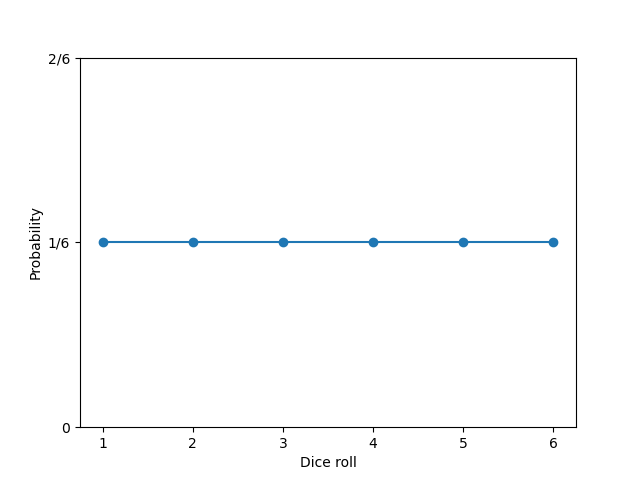
\includegraphics[width=.45\linewidth]{dice-plot.png}
 \end{center}
\end{frame}

\begin{frame}
 \frametitle{Visualizing Probability Distributions -- Graphs}
 The probability distribution from this table
 \begin{center}
  \begin{tabular}{c|cccc}
   \textbf{Value} & a & b & c & d\\
   \midrule
   \textbf{Probability} & $\frac{3}{10}$ & $\frac{5}{10}$ & $\frac{1}{10}$ &
   $\frac{1}{10}$.
  \end{tabular}
 \end{center}
 looks like this
 \vspace*{-1em}
 \begin{center}
  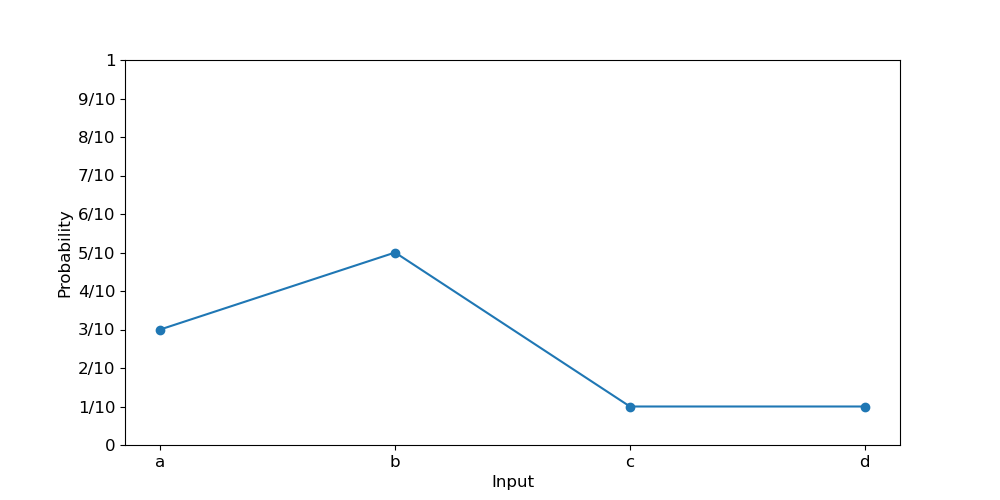
\includegraphics[width=.55\linewidth]{random-probability.png}
 \end{center}
\end{frame}

\subsection{Discrete Probability Distributions}

\begin{frame}
 \subsectionpage
\end{frame}

\begin{frame}
 \frametitle{Discrete Probability Distribution}
 Let $X$ be a random variable taking values from a set $A$.\pause
 \begin{itemize}
  \item The \alert{probability distribution} (or also \alert{probability mass
   function}) of $X$ is the function $f:A \to [0,1]$ defined as $f(a) = P(X =
   a)$ for $a \in A$. \pause
  \item The \alert{cumulative distribution function} of $X$ gives the
   probability that a random variable is \alert{less than a certain value}. It
   is defined as $F(a) = P(X \leq a)$ for $a \in A$. \pause
  \item The \alert{mean} of $X$ is defined as $E(X) = \sum_{a \in A} a \cdot P(X = a)$.
   It represents the `expected' value of $X$. \pause
  \item The \alert{variance} (describing the \emph{dispersion} of the
   distribution around the mean) of $X$ is defined as
   \[
    \var(X) = \sum_{a \in A} (a - E(X))^2 \cdot P(X = a).
   \]
 \end{itemize}
\end{frame}

\begin{frame}
 \frametitle{Discrete Probability Distribution -- Example}
 Let's see what these concepts mean in a simple statistical experiment.\\ \pause
 Suppose we measure the height of a randomly picked 20-year-old males. We might
 get something akin to the following table
 \begin{center}
  \begin{tabular}{c|ccccccccc}
   \textbf{Height} & 175 & 176 & 177 & 178 & 179 & 180 & 181 & 182 & 183\\
   \midrule
   \textbf{Count} & 13 & 20 & 11 & 17 & 11 & 8 & 10 & 7 & 3
  \end{tabular}
 \end{center}
 \pause
 We can easily calculate the mean and standard deviation of this data. 
\end{frame}

\begin{frame}
 \frametitle{Discrete Probability Distribution -- Example}
  \begin{center}
  \begin{tabular}{c|ccccccccc}
   \textbf{Height} & 175 & 176 & 177 & 178 & 179 & 180 & 181 & 182 & 183\\
   \midrule
   \textbf{Count} & 13 & 20 & 11 & 17 & 11 & 8 & 10 & 7 & 3
  \end{tabular}
 \end{center}
 Using the formula for the arithmetic mean, we get
 \[
  \bar{x} = \frac{175 \cdot 13 + 176 \cdot 20 + \ldots + 183 \cdot 3}{13 + 20 +
  \ldots + 3} = 178.1
 \]
\end{frame}

\begin{frame}
 \frametitle{Discrete Probability Distribution -- Example}
  \begin{center}
  \begin{tabular}{c|ccccccccc}
   \textbf{Height} & 175 & 176 & 177 & 178 & 179 & 180 & 181 & 182 & 183\\
   \midrule
   \textbf{Count} & 13 & 20 & 11 & 17 & 11 & 8 & 10 & 7 & 3
  \end{tabular}
 \end{center}
 The standard deviation is then
 \[
  \sigma = \sqrt{\frac{13 \cdot (175 - 178.1)^2 + 20 \cdot (176 - 178.1)^2 +
  \ldots + 3 \cdot (183 - 178.1)^2}{13 + 20 + \ldots + 3}} = 8.203.
 \]
\end{frame}

\begin{frame}
 \frametitle{Discrete Probability Distribution -- Example}
  \begin{center}
  \begin{tabular}{c|ccccccccc}
   \textbf{Height} & 175 & 176 & 177 & 178 & 179 & 180 & 181 & 182 & 183\\
   \midrule
   \textbf{Count} & 13 & 20 & 11 & 17 & 11 & 8 & 10 & 7 & 3
  \end{tabular}
 \end{center}
 Let's now define a random variable $X$ which can be any of those heights in the
 table above. \\ \pause
 We define the probabilities that $X$ is a particular height based on the counts
 above. That gives the following table
 \begin{center}
  \begin{tabular}{c|ccccccccc}
   \textbf{Height} & 175 & 176 & 177 & 178 & 179 & 180 & 181 & 182 & 183\\
   \midrule
   \textbf{Probability} & $\frac{13}{100}$ & $\frac{20}{100}$ & $\frac{11}{100}$
                        & $\frac{17}{100}$ & $\frac{11}{100}$ & $\frac{8}{100}$
                        & $\frac{10}{100}$ & $\frac{7}{100}$ & $\frac{3}{100}$
  \end{tabular}
 \end{center}
 \pause
 In other words, this gives a \alert{distribution function} $f$ of $X$ where the
 set $A = \{175, 176, 177, 178, 179, 180, 181, 182, 183\}$ and the outputs of
 $f$ on each of these numbers are given by the table above.
\end{frame}

\begin{frame}
 \frametitle{Discrete Probability Distribution -- Example}
 \begin{center}
  \begin{tabular}{c|ccccccccc}
   \textbf{Height} & 175 & 176 & 177 & 178 & 179 & 180 & 181 & 182 & 183\\
   \midrule
   \textbf{Probability} & $\frac{13}{100}$ & $\frac{20}{100}$ & $\frac{11}{100}$
                        & $\frac{17}{100}$ & $\frac{11}{100}$ & $\frac{8}{100}$
                        & $\frac{10}{100}$ & $\frac{7}{100}$ & $\frac{3}{100}$
  \end{tabular}
 \end{center}
 \begin{itemize}
  \item The \alert{cumulative distribution function} $F$ describes the
   probability that a randomly chosen person from the group has height
   \emph{less than} a particular number. \pause For example,
   \begin{align*}
    F(178) &= P(X \leq 178) = P(X = 175) + P(X = 176) + P(X = 177) + P(X =
    178)\\
           &= \frac{13}{100} + \frac{20}{100} + \frac{11}{100} + \frac{17}{100}
           = \frac{61}{100}.
   \end{align*}
 \end{itemize}
\end{frame}

\begin{frame}
 \frametitle{Discrete Probability Distribution -- Example}
 \begin{center}
  \begin{tabular}{c|ccccccccc}
   \textbf{Height} & 175 & 176 & 177 & 178 & 179 & 180 & 181 & 182 & 183\\
   \midrule
   \textbf{Probability} & $\frac{13}{100}$ & $\frac{20}{100}$ & $\frac{11}{100}$
                        & $\frac{17}{100}$ & $\frac{11}{100}$ & $\frac{8}{100}$
                        & $\frac{10}{100}$ & $\frac{7}{100}$ & $\frac{3}{100}$
  \end{tabular}
 \end{center}
 \begin{itemize}
  \item The \alert{mean} of $X$ is the same as the arithmetic mean of the data.
   Indeed,
   \begin{align*}
    E(X) &= \sum_{a \in A} a \cdot P(X = a)\\
         &= 175 \cdot P(X = 175) + 176 \cdot P(X = 176) + \ldots + 183 \cdot P(X
         = 183)\\
         &= 175 \cdot \frac{13}{100} + 176 \cdot \frac{20}{100} + \ldots + 183
         \cdot \frac{3}{100} = 178.1.
   \end{align*}
 \end{itemize}
\end{frame}

\begin{frame}
 \frametitle{Discrete Probability Distribution -- Example}
 \begin{center}
  \begin{tabular}{c|ccccccccc}
   \textbf{Height} & 175 & 176 & 177 & 178 & 179 & 180 & 181 & 182 & 183\\
   \midrule
   \textbf{Probability} & $\frac{13}{100}$ & $\frac{20}{100}$ & $\frac{11}{100}$
                        & $\frac{17}{100}$ & $\frac{11}{100}$ & $\frac{8}{100}$
                        & $\frac{10}{100}$ & $\frac{7}{100}$ & $\frac{3}{100}$
  \end{tabular}
 \end{center}
 \begin{itemize}
  \item The \alert{variance} of $X$ is the same as the standard deviation
   \emph{squared} (that is, $\var(X) = \sigma^2$). Indeed,
   \begin{align*}
    \var(X) &= \sum_{a \in A} (a - E(X))^2 \cdot P(X = a)\\
            &= (175 - 178.1)^2 \cdot P(X = 175) + \ldots + (183 - 178.1)^2 \cdot
            P(X = 183)\\
            &= 67.29 = 8.203^2.
   \end{align*}
 \end{itemize}
\end{frame}

\section{Some Important Discrete Distributions}

\begin{frame}
 \frametitle{The Bernoulli Distribution}
 The \alert{Bernoulli} distribution is a discrete distribution of a random
 variable which can only attain \alert{two distinct values}.\\ \pause
 If we denote these values as $0$ and $1$, then the Bernoulli distribution is
 the function
 \[
  f(x) = \begin{cases}
   p, \quad &\text{if } x = 1,\\
   1 - p, \quad &\text{if } x = 0,
  \end{cases}
 \]
 where $p \in [0,1]$ is a \alert{fixed} probability.
\end{frame}

\begin{frame}
 \frametitle{The Bernoulli Distribution -- Example}
 A \alert{coin toss} is a perfect example of a Bernoulli distribution with $p =
 1 / 2$. \\ \pause
 Indeed, if $f$ is the probability distribution of the result of a coin toss,
 then
 \[
  f(x) = 
  \begin{cases}
   \frac{1}{2}, \quad &\text{if } x = \text{heads},\\
   \frac{1}{2}, \quad &\text{if } x = \text{tails}.
  \end{cases}
 \]
\end{frame}

\begin{frame}
 \frametitle{The Bernoulli Distribution -- Properties}
 We compute the distribution, cumulative distribution, mean and variance of the
 Bernoulli distribution. We assume that $X \in \{0,1\}$ and $p \in [0,1]$.\\
 \pause
 \begin{itemize}
  \item By definition, $f(1) = p$ and $f(0) = 1 - p$. \pause
  \item Since we have only two values, $F(0) = P(X \leq 0) = P(X = 0) = f(0) = 1
   - p$ and $F(1) = P(X \leq 1) = f(0) + f(1) = 1$. \pause
  \item We calculate,
  \[
   E(X) = \sum_{a \in \{0,1\}} a \cdot f(a) = 0 \cdot f(0) + 1 \cdot f(1) = 0
   \cdot (1-p) + 1 \cdot p = p.
  \]
  \pause
 \item And also
 \[
  \var(X) = \sum_{a \in \{0,1\}} (a - E(X))^2 \cdot f(a) = (0 - p)^2 \cdot (1-p)
  + (1 - p)^2 \cdot p = p(1-p).
 \]
 \end{itemize}
\end{frame}

\subsection{Digression\\ $\big\downarrow$ \\ Variations \& Combinations}

\begin{frame}
 \subsectionpage
\end{frame}

\begin{frame}
 \frametitle{How To Count The Number Of Repetitions?}
 Imagine 11 people standing in supermarket queue. How many different ways can
 they order themselves in that queue?\\ \pause
 The answer is relatively simple.\\ \pause
 Imagine 11 empty boxes and count how many ways can you distribute 11 people
 into them.
 \begin{center}
  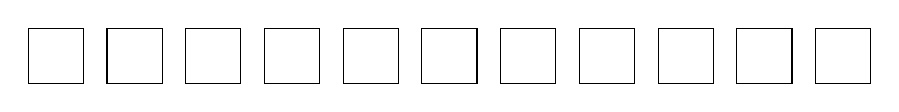
\begin{tikzpicture}
   \node[draw,rectangle,minimum width=7mm,minimum height=7mm] at (0,0) {};
   \node[draw,rectangle,minimum width=7mm,minimum height=7mm] at (1,0) {};
   \node[draw,rectangle,minimum width=7mm,minimum height=7mm] at (2,0) {};
   \node[draw,rectangle,minimum width=7mm,minimum height=7mm] at (3,0) {};
   \node[draw,rectangle,minimum width=7mm,minimum height=7mm] at (4,0) {};
   \node[draw,rectangle,minimum width=7mm,minimum height=7mm] at (5,0) {};
   \node[draw,rectangle,minimum width=7mm,minimum height=7mm] at (6,0) {};
   \node[draw,rectangle,minimum width=7mm,minimum height=7mm] at (7,0) {};
   \node[draw,rectangle,minimum width=7mm,minimum height=7mm] at (8,0) {};
   \node[draw,rectangle,minimum width=7mm,minimum height=7mm] at (9,0) {};
   \node[draw,rectangle,minimum width=7mm,minimum height=7mm] at (10,0) {};
  \end{tikzpicture}
 \end{center}
\end{frame}

\begin{frame}
 \frametitle{How To Count The Number Of Repetitions?}
 \begin{center}
  \begin{tikzpicture}
   \node (h1) at (0,4) {
\includegraphics[width=5mm]{human.png}};
   \node (h2) at (1,4) {
\includegraphics[width=5mm]{human.png}};
   \node (h3) at (2,4) {
\includegraphics[width=5mm]{human.png}};
   \node (h4) at (3,4) {
\includegraphics[width=5mm]{human.png}};
   \node (h5) at (4,4) {
\includegraphics[width=5mm]{human.png}};
   \node (h6) at (5,4) {
\includegraphics[width=5mm]{human.png}};
   \node (h7) at (6,4) {
\includegraphics[width=5mm]{human.png}};
   \node (h8) at (7,4) {
\includegraphics[width=5mm]{human.png}};
   \node (h9) at (8,4) {
\includegraphics[width=5mm]{human.png}};
   \node (h10) at (9,4) {
\includegraphics[width=5mm]{human.png}};
   \node (h11) at (10,4) {
\includegraphics[width=5mm]{human.png}};

   \node[draw,rectangle,minimum width=7mm,minimum height=7mm] (b1) at (0,0) {};
   \node[draw,rectangle,minimum width=7mm,minimum height=7mm] (b2) at (1,0) {};
   \node[draw,rectangle,minimum width=7mm,minimum height=7mm] (b3) at (2,0) {};
   \node[draw,rectangle,minimum width=7mm,minimum height=7mm] (b4) at (3,0) {};
   \node[draw,rectangle,minimum width=7mm,minimum height=7mm] (b5) at (4,0) {};
   \node[draw,rectangle,minimum width=7mm,minimum height=7mm] (b6) at (5,0) {};
   \node[draw,rectangle,minimum width=7mm,minimum height=7mm] (b7) at (6,0) {};
   \node[draw,rectangle,minimum width=7mm,minimum height=7mm] (b8) at (7,0) {};
   \node[draw,rectangle,minimum width=7mm,minimum height=7mm] (b9) at (8,0) {};
   \node[draw,rectangle,minimum width=7mm,minimum height=7mm] (b10) at (9,0) {};
   \node[draw,rectangle,minimum width=7mm,minimum height=7mm] (b11) at (10,0) {};

   \draw[-latex,thick,shorten >=2pt] (h1.south) -- (b4.north);
   \draw[-latex,thick,shorten >=2pt] (h2.south) -- (b6.north);
   \draw[-latex,thick,shorten >=2pt] (h3.south) -- (b1.north);
   \draw[-latex,thick,shorten >=2pt] (h4.south) -- (b11.north);
   \draw[-latex,thick,shorten >=2pt] (h5.south) -- (b5.north);
   \draw[-latex,thick,shorten >=2pt] (h6.south) -- (b3.north);
   \draw[-latex,thick,shorten >=2pt] (h7.south) -- (b8.north);
   \draw[-latex,thick,shorten >=2pt] (h8.south) -- (b9.north);
   \draw[-latex,thick,shorten >=2pt] (h9.south) -- (b2.north);
   \draw[-latex,thick,shorten >=2pt] (h10.south) -- (b7.north);
   \draw[-latex,thick,shorten >=2pt] (h11.south) -- (b10.north);
  \end{tikzpicture}
 \end{center}
\end{frame}

\begin{frame}
 \frametitle{How To Count The Number Of Repetitions?}
 \begin{center}
  \begin{tikzpicture}
   \node (h1) at (0,4) {
\includegraphics[width=5mm]{human.png}};
   \node (h2) at (1,4) {
\includegraphics[width=5mm]{human.png}};
   \node (h3) at (2,4) {
\includegraphics[width=5mm]{human.png}};
   \node (h4) at (3,4) {
\includegraphics[width=5mm]{human.png}};
   \node (h5) at (4,4) {
\includegraphics[width=5mm]{human.png}};
   \node (h6) at (5,4) {
\includegraphics[width=5mm]{human.png}};
   \node (h7) at (6,4) {
\includegraphics[width=5mm]{human.png}};
   \node (h8) at (7,4) {
\includegraphics[width=5mm]{human.png}};
   \node (h9) at (8,4) {
\includegraphics[width=5mm]{human.png}};
   \node (h10) at (9,4) {
\includegraphics[width=5mm]{human.png}};
   \node (h11) at (10,4) {
\includegraphics[width=5mm]{human.png}};

   \node[draw,rectangle,minimum width=7mm,minimum height=7mm] (b1) at (0,0) {};
   \node[draw,rectangle,minimum width=7mm,minimum height=7mm] (b2) at (1,0) {};
   \node[draw,rectangle,minimum width=7mm,minimum height=7mm] (b3) at (2,0) {};
   \node[draw,rectangle,minimum width=7mm,minimum height=7mm] (b4) at (3,0) {};
   \node[draw,rectangle,minimum width=7mm,minimum height=7mm] (b5) at (4,0) {};
   \node[draw,rectangle,minimum width=7mm,minimum height=7mm] (b6) at (5,0) {};
   \node[draw,rectangle,minimum width=7mm,minimum height=7mm] (b7) at (6,0) {};
   \node[draw,rectangle,minimum width=7mm,minimum height=7mm] (b8) at (7,0) {};
   \node[draw,rectangle,minimum width=7mm,minimum height=7mm] (b9) at (8,0) {};
   \node[draw,rectangle,minimum width=7mm,minimum height=7mm] (b10) at (9,0) {};
   \node[draw,rectangle,minimum width=7mm,minimum height=7mm] (b11) at (10,0) {};

   \draw[-latex,thick,shorten >=2pt] (h1.south) -- (b2.north);
   \draw[-latex,thick,shorten >=2pt] (h2.south) -- (b3.north);
   \draw[-latex,thick,shorten >=2pt] (h3.south) -- (b4.north);
   \draw[-latex,thick,shorten >=2pt] (h4.south) -- (b5.north);
   \draw[-latex,thick,shorten >=2pt] (h5.south) -- (b6.north);
   \draw[-latex,thick,shorten >=2pt] (h6.south) -- (b7.north);
   \draw[-latex,thick,shorten >=2pt] (h7.south) -- (b8.north);
   \draw[-latex,thick,shorten >=2pt] (h8.south) -- (b9.north);
   \draw[-latex,thick,shorten >=2pt] (h9.south) -- (b10.north);
   \draw[-latex,thick,shorten >=2pt] (h10.south) -- (b11.north);
   \draw[-latex,thick,shorten >=2pt] (h11.south) -- (b1.north);
  \end{tikzpicture}
 \end{center}
\end{frame}

\begin{frame}
 \frametitle{How To Count The Number Of Repetitions?}
 What if there were only $1$ human? \pause
 \begin{center}
  \begin{tikzpicture}[scale=0.75,every node/.style={transform shape}]
   \node (h1) at (5,4) {
\includegraphics[width=5mm]{human.png}};

   \node[draw,rectangle,minimum width=7mm,minimum height=7mm] (b1) at (0,0) {};
   \node[draw,rectangle,minimum width=7mm,minimum height=7mm] (b2) at (1,0) {};
   \node[draw,rectangle,minimum width=7mm,minimum height=7mm] (b3) at (2,0) {};
   \node[draw,rectangle,minimum width=7mm,minimum height=7mm] (b4) at (3,0) {};
   \node[draw,rectangle,minimum width=7mm,minimum height=7mm] (b5) at (4,0) {};
   \node[draw,rectangle,minimum width=7mm,minimum height=7mm] (b6) at (5,0) {};
   \node[draw,rectangle,minimum width=7mm,minimum height=7mm] (b7) at (6,0) {};
   \node[draw,rectangle,minimum width=7mm,minimum height=7mm] (b8) at (7,0) {};
   \node[draw,rectangle,minimum width=7mm,minimum height=7mm] (b9) at (8,0) {};
   \node[draw,rectangle,minimum width=7mm,minimum height=7mm] (b10) at (9,0) {};
   \node[draw,rectangle,minimum width=7mm,minimum height=7mm] (b11) at (10,0) {};

   \draw[-latex,thick,dashed,color=RoyalBlue,shorten >=2pt] (h1.south) -- (b1.north);
   \draw[-latex,thick,dashed,color=RoyalBlue,shorten >=2pt] (h1.south) -- (b2.north);
   \draw[-latex,thick,dashed,color=RoyalBlue,shorten >=2pt] (h1.south) -- (b3.north);
   \draw[-latex,thick,dashed,color=RoyalBlue,shorten >=2pt] (h1.south) -- (b4.north);
   \draw[-latex,thick,dashed,color=RoyalBlue,shorten >=2pt] (h1.south) -- (b5.north);
   \draw[-latex,thick,dashed,color=RoyalBlue,shorten >=2pt] (h1.south) -- (b6.north);
   \draw[-latex,thick,dashed,color=RoyalBlue,shorten >=2pt] (h1.south) -- (b7.north);
   \draw[-latex,thick,dashed,color=RoyalBlue,shorten >=2pt] (h1.south) -- (b8.north);
   \draw[-latex,thick,dashed,color=RoyalBlue,shorten >=2pt] (h1.south) -- (b9.north);
   \draw[-latex,thick,dashed,color=RoyalBlue,shorten >=2pt] (h1.south) -- (b10.north);
   \draw[-latex,thick,dashed,color=RoyalBlue,shorten >=2pt] (h1.south) -- (b11.north);
  \end{tikzpicture}
 \end{center}
 \pause
 I'd have exactly 11 options where to put him.
\end{frame}

\begin{frame}
 \frametitle{How To Count The Number Of Repetitions?}
 So, I put him in a random box and in comes the second human.\pause
 \begin{center}
  \begin{tikzpicture}[scale=1,every node/.style={transform shape}]
   \node (h1) at (5,4) {
\includegraphics[width=5mm]{human.png}};

   \node[draw,rectangle,minimum width=7mm,minimum height=7mm] (b1) at (0,0) {};
   \node[draw,rectangle,minimum width=7mm,minimum height=7mm] (b2) at (1,0) {};
   \node[draw,rectangle,minimum width=7mm,minimum height=7mm] (b3) at (2,0) {};
   \node[draw,rectangle,minimum width=7mm,minimum height=7mm] (b4) at (3,0) {};
   \node[draw,thick,rectangle,minimum width=7mm,minimum height=7mm,color=RoyalBlue]
    (b5) at (4,0) {
\includegraphics[width=2mm]{human.png}};
   \node[draw,rectangle,minimum width=7mm,minimum height=7mm] (b6) at (5,0) {};
   \node[draw,rectangle,minimum width=7mm,minimum height=7mm] (b7) at (6,0) {};
   \node[draw,rectangle,minimum width=7mm,minimum height=7mm] (b8) at (7,0) {};
   \node[draw,rectangle,minimum width=7mm,minimum height=7mm] (b9) at (8,0) {};
   \node[draw,rectangle,minimum width=7mm,minimum height=7mm] (b10) at (9,0) {};
   \node[draw,rectangle,minimum width=7mm,minimum height=7mm] (b11) at (10,0) {};

   \draw[-latex,thick,dashed,color=BrickRed,shorten >=2pt] (h1.south) -- (b1.north);
   \draw[-latex,thick,dashed,color=BrickRed,shorten >=2pt] (h1.south) -- (b2.north);
   \draw[-latex,thick,dashed,color=BrickRed,shorten >=2pt] (h1.south) -- (b3.north);
   \draw[-latex,thick,dashed,color=BrickRed,shorten >=2pt] (h1.south) -- (b4.north);
   \draw[-latex,thick,dashed,color=BrickRed,shorten >=2pt] (h1.south) -- (b6.north);
   \draw[-latex,thick,dashed,color=BrickRed,shorten >=2pt] (h1.south) -- (b7.north);
   \draw[-latex,thick,dashed,color=BrickRed,shorten >=2pt] (h1.south) -- (b8.north);
   \draw[-latex,thick,dashed,color=BrickRed,shorten >=2pt] (h1.south) -- (b9.north);
   \draw[-latex,thick,dashed,color=BrickRed,shorten >=2pt] (h1.south) -- (b10.north);
   \draw[-latex,thick,dashed,color=BrickRed,shorten >=2pt] (h1.south) -- (b11.north);
  \end{tikzpicture}
 \end{center}
 \pause
 I'd have only 10 boxes left to place him into.
\end{frame}

\begin{frame}
 \frametitle{How To Count The Number Of Repetitions?}
 For the third human, only 9 boxes are left, etc.
 \begin{center}
  \begin{tikzpicture}[scale=1,every node/.style={transform shape}]
   \node (h1) at (5,4) {
\includegraphics[width=5mm]{human.png}};

   \node[draw,rectangle,minimum width=7mm,minimum height=7mm] (b1) at (0,0) {};
   \node[draw,rectangle,minimum width=7mm,minimum height=7mm] (b2) at (1,0) {};
   \node[draw,rectangle,minimum width=7mm,minimum height=7mm] (b3) at (2,0) {};
   \node[draw,rectangle,minimum width=7mm,minimum height=7mm] (b4) at (3,0) {};
   \node[draw,thick,rectangle,minimum width=7mm,minimum
   height=7mm,color=RoyalBlue] (b5) at (4,0)
   {
\includegraphics[width=2mm]{human.png}};
   \node[draw,rectangle,minimum width=7mm,minimum height=7mm] (b6) at (5,0) {};
   \node[draw,rectangle,minimum width=7mm,minimum height=7mm] (b7) at (6,0) {};
   \node[draw,thick,rectangle,minimum width=7mm,minimum
   height=7mm,color=BrickRed] (b8) at (7,0)
   {
\includegraphics[width=2mm]{human.png}};
   \node[draw,rectangle,minimum width=7mm,minimum height=7mm] (b9) at (8,0) {};
   \node[draw,rectangle,minimum width=7mm,minimum height=7mm] (b10) at (9,0) {};
   \node[draw,rectangle,minimum width=7mm,minimum height=7mm] (b11) at (10,0) {};

   \draw[-latex,thick,dashed,color=ForestGreen,shorten >=2pt] (h1.south) -- (b1.north);
   \draw[-latex,thick,dashed,color=ForestGreen,shorten >=2pt] (h1.south) -- (b2.north);
   \draw[-latex,thick,dashed,color=ForestGreen,shorten >=2pt] (h1.south) -- (b3.north);
   \draw[-latex,thick,dashed,color=ForestGreen,shorten >=2pt] (h1.south) -- (b4.north);
   \draw[-latex,thick,dashed,color=ForestGreen,shorten >=2pt] (h1.south) -- (b6.north);
   \draw[-latex,thick,dashed,color=ForestGreen,shorten >=2pt] (h1.south) -- (b7.north);
   \draw[-latex,thick,dashed,color=ForestGreen,shorten >=2pt] (h1.south) -- (b9.north);
   \draw[-latex,thick,dashed,color=ForestGreen,shorten >=2pt] (h1.south) -- (b10.north);
   \draw[-latex,thick,dashed,color=ForestGreen,shorten >=2pt] (h1.south) -- (b11.north);
  \end{tikzpicture}
 \end{center}
\end{frame}

\begin{frame}
 \frametitle{Factorial}
 \begin{tcolorbox}[title=Factorial]
  Overall, given $n$ objects, I have
  \[
   n \cdot (n-1) \cdot (n-2) \cdot \ldots \cdot 1
  \]
  ways how to order them. This number is written as $n!$ and read \alert{$n$
  factorial}.
 \end{tcolorbox}
\end{frame}

\begin{frame}
 \frametitle{What If I Have Fewer Boxes?}
 \begin{center}
  \begin{tikzpicture}
   \node (h1) at (0,4) {
\includegraphics[width=5mm]{human.png}};
   \node (h2) at (1,4) {
\includegraphics[width=5mm]{human.png}};
   \node (h3) at (2,4) {
\includegraphics[width=5mm]{human.png}};
   \node (h4) at (3,4) {
\includegraphics[width=5mm]{human.png}};
   \node (h5) at (4,4) {
\includegraphics[width=5mm]{human.png}};
   \node (h6) at (5,4) {
\includegraphics[width=5mm]{human.png}};
   \node (h7) at (6,4) {
\includegraphics[width=5mm]{human.png}};
   \node (h8) at (7,4) {
\includegraphics[width=5mm]{human.png}};
   \node (h9) at (8,4) {
\includegraphics[width=5mm]{human.png}};
   \node (h10) at (9,4) {
\includegraphics[width=5mm]{human.png}};
   \node (h11) at (10,4) {
\includegraphics[width=5mm]{human.png}};

   \node[draw,rectangle,minimum width=7mm,minimum height=7mm] (b1) at (3,0) {};
   \node[draw,rectangle,minimum width=7mm,minimum height=7mm] (b2) at (4,0) {};
   \node[draw,rectangle,minimum width=7mm,minimum height=7mm] (b3) at (5,0) {};
   \node[draw,rectangle,minimum width=7mm,minimum height=7mm] (b4) at (6,0) {};
   \node[draw,rectangle,minimum width=7mm,minimum height=7mm] (b5) at (7,0) {};

   \draw[-latex,thick,shorten >=2pt] (h1.south) -- (b4.north);
   \draw[-latex,thick,shorten >=2pt] (h3.south) -- (b1.north);
   \draw[-latex,thick,shorten >=2pt] (h5.south) -- (b5.north);
   \draw[-latex,thick,shorten >=2pt] (h6.south) -- (b3.north);
   \draw[-latex,thick,shorten >=2pt] (h9.south) -- (b2.north);
  \end{tikzpicture}
 \end{center}
\end{frame}

\begin{frame}
 \frametitle{What If I Have Fewer Boxes?}
 The same argument applies.\\ \pause
 If I have only 5 boxes and 11 humans, I have
 \[
  11 \cdot 10 \cdot 9 \cdot 8 \cdot 7
 \]
 ways to put 5 of those humans into all the boxes.\pause
 \begin{tcolorbox}[title=Variations]
  If I have $n$ elements, the number of ways how to order any $k$ of them is
  \[
   n \cdot (n-1) \cdot (n-2) \cdot \ldots \cdot (n-k+1) = \frac{n!}{(n-k)!}.
  \]
  This number is sometimes called the number of \alert{variations} of $k$
  elements out of $n$.
 \end{tcolorbox}
\end{frame}

\begin{frame}
 \frametitle{What If I Don't Care About The Order?}
 Finally, suppose I'm not interested in the differences between individual
 humans and I just want to place some 5 of them into boxes.\\ \pause
 In other words, I don't care about the order I put them into those boxes. It
 doesn't matter to me which human goes to which box as long as all the boxes are
 full.\\ \pause
 This is a similar problem. The only difference is that I disregard all the ways
 I can order those $k$ elements inside the boxes.
\end{frame}

\begin{frame}
 \frametitle{Combinations}
 \begin{tcolorbox}[title=Combinations]
  If I have $n$ elements, the number of ways I can choose any $k$ of them
  regardless of order, is
  \[
   \frac{n \cdot (n-1) \cdot (n-2) \cdot \ldots \cdot (n-k+1)}{k!} =
   \frac{n!}{(n-k)!k!}.
  \]
  This number is typically written as $\binom{n}{k}$ and read `\alert{$n$ choose
  $k$}'.
 \end{tcolorbox}
\end{frame}

\subsection{The Binomial Distribution}

\begin{frame}
 \subsectionpage
\end{frame}

\begin{frame}
 \frametitle{The Binomial Distribution}
 The \alert{binomial distribution} describes the probability of multiple
 occurrences whose probabilities are given by the Bernoulli distribution.\\
 \pause
 Common examples include
 \begin{itemize}
  \item What's the probability that 7 out of 10 coin tosses are heads?
  \item What's the probability that 60 out of 100 people are male?
 \end{itemize}
\end{frame}

\begin{frame}
 \frametitle{The Binomial Distribution}
 Let's think about how to calculate this probability in the example of `7 out of
 10 coin tosses'.\\ \pause
 One would think the probability is just $(1 / 2)^{7} \cdot (1 / 2)^{3}$, that
 is, the probability that I get 7 heads in a row and then 3 tails.\\ \pause
 But, that is \alert{not correct} because the 7 heads don't necessarily come one
 after another. \pause Here are a few examples of a `positive' outcome:
 \begin{align*}
  & HHHHHHHTTT,\\
  & THHTTHHHHH,\\
  & HHHTHHTHTH,\\
  & \hspace{5.5ex} \vdots
 \end{align*}
\end{frame}

\begin{frame}
 \frametitle{The Binomial Distribution}
 The number $(1 / 2)^{7} \cdot (1 / 2)^3$ is the probability of \alert{just one
 such occurrence}.\\ \pause
 How many possible occurrences of 7 heads in 10 coin tosses are there?\\ \pause
 The answer is $\binom{10}{7}$ -- the number of ways one can choose 7 objects
 out of 10.\\ \pause
 Therefore, the \alert{actual probability} of getting 7 heads in 10 coin tosses
 is 
 \[
  \binom{10}{7} \cdot \left( \frac{1}{2} \right)^{7} \cdot \left( \frac{1}{2}
  \right)^3.
 \]
\end{frame}

\begin{frame}
 \frametitle{The Binomial Distribution}
 \begin{tcolorbox}[title=Def\hspace{0pt}inition]
  If $X$ is a random variable with \alert{Bernoulli distribution} with
  probability $p$, the probability that $X = x$ exactly $k$ times out of $n$ is
  \[
   f(x) = \binom{n}{k} \cdot p^{k} \cdot (1-p)^{n-k}.
  \]
 \end{tcolorbox}
\end{frame}

\begin{frame}
 \frametitle{The Binomial Distribution -- Problems}
 Let’s say that 80 \% of all business startups in the IT industry report that
 they generate a profit in their first year. If a sample of 10 new IT business
 startups is selected, find the probability that exactly seven will generate a
 profit in their first year.
\end{frame}

\begin{frame}
 \frametitle{The Binomial Distribution -- Problems}
 Your basketball team is playing a series of 5 games against your opponent. The winner is those who wins more games (out of 5).

 Let assume that your team is much more skilled and has 75 \% chances of winning.
 It means there is a 25 \% chance of losing.

 What is the probability of your team get 3 wins?
\end{frame}

\begin{frame}
 \frametitle{The Binomial Distribution -- Problems}
 A box of candies has many different colors in it. There is a 15 \% chance of
 getting a pink candy. What is the probability that exactly 4 candies in a box
 are pink out of 10?
\end{frame}

\begin{frame}
 \frametitle{The Binomial Distribution -- Properties}
 The probability distribution of $k$ successes out of $n$ tries with probability
 of success $p$ is called the \alert{binomial distribution} with parameter
 $n$.\\ \pause
 It has the following properties (here, $X$ is a random variable representing
 the number of successes).
 \vspace*{-1em}
 \begin{align*}
  f(x) &= P(X = k) = \binom{n}{k} p^{k} (1-p)^{n-k},\\
  F(x) &= P(X \leq k) = \sum_{a=0}^k \binom{n}{k} p^{k}(1-p)^{n-k},\\
  E(X) &= \sum_{k=0}^n k \cdot f(k) = \sum_{k=0}^n k \cdot \binom{n}{k}
  p^{k}(1-p)^{n-k} = n \cdot p,\\
  \var(X) &= \sum_{k=0}^n (k-E(X))^2 \cdot f(k) = n \cdot p \cdot (1-p).
 \end{align*}
\end{frame}

\begin{frame}
 \frametitle{The Multinomial Distribution}
 The final `\alert{upgrade}' 
\end{frame}

\end{document}
